% !TEX program = xelatex

\documentclass[a4paper,12pt]{article}

\usepackage[ngerman]{babel} % Deutsche Sonderzeichen und Silbentrennung nutzen
\usepackage[german]{nomencl} % Erstellen von Listen (Nomenklaturen)
\usepackage{fontspec} % Zeichenencoding
\usepackage[hyphens]{url} % bricht lange URLs "schön" um // aber nur mit der Option Moritz ;-)
\usepackage{graphicx} % Grafiken aus PNG Dateien einbinden
\usepackage{rotating} % um große grafiken zu drehen
\usepackage[right]{eurosym} % Eurozeichen einbinden
\usepackage{longtable} % mehrseitige Tabellen ermöglichen
\usepackage{color} % Paket für Textfarben
\usepackage{amssymb} % Mathematische Symbole importieren
\usepackage{array} % für Tabellen
\usepackage{blindtext} % Um Blindtext als Beispiel zu erstellen
\usepackage[dvipsnames,table,xcdraw]{xcolor}
\usepackage{amsmath} % Für Formeln und Formelverzeichnis
\usepackage[backend=biber, sorting=none, citestyle=ieee]{biblatex} % Für Zitate
\usepackage{csquotes} % Für babel
\usepackage[hidelinks]{hyperref} % Für Links intern und extern
\usepackage{multirow} % Tabelle mit zusammengefügten Zeilen
\usepackage{wrapfig} % Textumflossene Grafik
\usepackage{caption} % Passe deine Bild- Tabellen-, etc. -überschriften an. 
\usepackage{subcaption} % Zum Einbinden von Subfigs und Subcaptions
\usepackage{setspace} % Paket für Zeilenabstand
\usepackage{fancyhdr} % Für Kopf- und Fußzeilen
\usepackage{geometry} % Packet für Seitenrandabständex und Einstellung für Seitenränder
\usepackage{float}
\usepackage{listings}

\usepackage{placeins} % für FlotBarrierer

% For rotating figures, tables, etc.
%  including their captions
\usepackage{rotating}

 \usepackage{booktabs}
 \usepackage[table,xcdraw]{xcolor}
% If you use beamer only pass "xcolor=table" option, i.e. \documentclass[xcolor=table]{beamer}
 \usepackage{longtable}


% Ohne Einrückung bei neuem Absatz
\setlength{\parindent}{0pt}

% Festlegung Art der Zitierung
\addbibresource{LiteraturVerzeichnis/Literatur.bib}

% Abkürzungsverezichnis
\usepackage[printonlyused]{acronym}

% Setup Captions
\captionsetup[wrapfigure]{format=plain}

\usepackage[absolute]{textpos} %Um Objekte Absolut auf einer Seite zu positionieren benutzt für das HTW Logo

% Geometrie des Dokuments
\geometry{left=3cm, right=2.5cm, top=2.5cm, bottom=2.5cm}

% Neue Kopfzeilen mit dem Paket fancyhdr
\setlength{\headheight}{15pt} % Warnung headhight is too small. 
\pagestyle{fancy} %eigener Seitenstil
\fancyhf{} %alle Kopf- und Fußzeilenfelder bereinigen
\fancyhead[L]{\nouppercase{\leftmark}} %Kopfzeile links
\fancyhead[C]{} %zentrierte Kopfzeile
\fancyhead[R]{\thepage} %Kopfzeile rechts
\renewcommand{\headrulewidth}{0.4pt} %obere Trennlinie

% for subplots (images)
\usepackage{subcaption}
% suppress floating tables and images
% use [H] to suppress
\usepackage{float}
% usage:
% \singlefigure{abb/image.png}{this is a cation}{fig:some_label}
\newcommand{\singlefigure}[3]{
	\begin{figure}[H]
		\centering
		%\includegraphics[width=1\textwidth]{images/RIFB.png}
		\includegraphics[height=10cm, keepaspectratio=true]{#1}
		\caption{#2}
		\label{#3}
	\end{figure}
}
% usage:
% \singlefigure{abb/image.png}{this is a cation}{fig:some_label}
\newcommand{\doublefigure}[6]{
	\begin{figure}[H]
		\centering
		\begin{subfigure}[b]{.5\textwidth}
			\centering
			%\includegraphics[width=0.9\textwidth]{#1}
			\includegraphics[height=10cm]{#1}
			\caption{#2}
		\end{subfigure}%
		\begin{subfigure}[b]{.5\textwidth}
			\centering
			%\includegraphics[width=0.9\textwidth]{#3}
			\includegraphics[height=10cm]{#3}
			\caption{#4}
		\end{subfigure}
		\caption{#5}
		\label{#6}
	\end{figure}
}

\newcommand{\inquote}[1]{
	\glqq{#1}\grqq{}
}


\definecolor{codegreen}{rgb}{0,0.6,0}
\definecolor{codegray}{rgb}{0.5,0.5,0.5}
\definecolor{codepurple}{rgb}{0.58,0,0.82}
\definecolor{backcolour}{rgb}{0.95,0.95,0.92}

\lstdefinestyle{mystyle}{
	backgroundcolor=\color{backcolour},   
	commentstyle=\color{codegreen},
	keywordstyle=\color{magenta},
	numberstyle=\tiny\color{codegray},
	stringstyle=\color{codepurple},
	basicstyle=\ttfamily\footnotesize,
	breakatwhitespace=false,         
	breaklines=true,                 
	captionpos=b,                    
	keepspaces=true,                 
	numbers=left,                    
	numbersep=5pt,                  
	showspaces=false,                
	showstringspaces=false,
	showtabs=false,                  
	tabsize=2
}

\lstset{style=mystyle}

%Einblenden der Seitenränder als Entwurfshilfe
%\usepackage{showframe}

% Begin Dokument =============================================================
\begin{document}

%Deckplatt
\thispagestyle{empty}
%Logos Kopfzeile
%\begin{tabbing}	\hspace{10.5cm}\=\kill
%	\includegraphics[height=55pt]{abb/Q04_HTW_Berlin_Logo_quer_pos_FARBIG_RGB.jpg} 
%	\> \includegraphics[height=45pt]{abb/Detecon_Logo_blau_72dpi_low_res.png}	
%\end{tabbing}

\begin{verbatim}
\end{verbatim}
\begin{center}
	\doublespacing
	\LARGE{Hochschule für Technik und Wirtschaft - Berlin}
	\singlespacing
	\textbf{\Large{Fachbereich 2\\  Ingenieurwissenschaften - Technik und Leben \\im Studiengang Ingenieurinformatik}}
\end{center}
\begin{verbatim}
	
\end{verbatim}
\begin{center}
	\doublespacing
	\textbf{\Large{Technische Dokumentation}}\\
	\singlespacing
\end{center}
\begin{verbatim}
	
\end{verbatim}
\begin{center}
	\Large{Einrichtung von OPC UA mit open62541} 	\\
	\Large{auf einem Raspberry Pi 4}\\
\end{center}
\begin{verbatim}
	
\end{verbatim}
\begin{center}
	Dieses Dokument dient als Anhang einer Bachelor Arbeit, \\ unterliegt allerdings nicht dessen Sperrvermerk
\end{center} 
\begin{tabbing}
	\hspace{5cm}\=\kill
	\textbf{Thema:}	\> Umsetzung der digitalen Durchgängigkeit \\ \> im Product   Lifecycle Management   (PLM) \\ \> mittels MBSE und OPC UA
\end{tabbing} 
\begin{tabbing}
	\hspace{5cm}\=\kill
	\textbf{Autor:}	\> Klemens Körner
\end{tabbing} 
\begin{tabbing}
	\hspace{5cm}\=\kill
	\textbf{Version vom:}	\> 19.04.2021
\end{tabbing} 
\clearpage

\pagenumbering{Roman}
\setcounter{page}{1}

% Inhaltsverzeichnis
\setcounter{tocdepth}{2} % Nur Section und Subsection im Inhaltsverzeichnis anzeigen
\tableofcontents
\clearpage

% Abbildungsverzeichnis
\addcontentsline{toc}{section}{Abbildungsverzeichnis} % Abbildungsverzeichnis im Inhaltsverzeichnis anzeigen
\listoffigures
\clearpage

% Tabellenverzeichnis
\addcontentsline{toc}{section}{Tabellenverzeichnis} % Tabellenverzeichnis im Inhaltsverzeichnis anzeigen
\listoftables
\clearpage

\input{Kapitel/04_Abkürzungsverzeichnis}
\clearpage

% Begin Des Inhalts ==========================================================
\pagenumbering{arabic}
\newgeometry{left=3.0cm, right=2.5cm, top=2.5cm, bottom=2.5cm}
\onehalfspacing

\section{Einleitung} \label{sec:einleitung}
Diese Technische Dokumentation dient als Anleitung zur Einrichtung eines OPC UA Servers auf einem Raspberry Pi4. Als Basis dient hierbei die Open Source-Variante von OPC UA open62541. Um das Verständnis dieser Dokumentation zu erhöhen, wird empfohlen, die dazugehörige Bachelor-Arbeit zu lesen. Dort werden sehr viele Informationen aus den Übungen von \url{https://opcua.rocks/} verarbeitet. Diese Seite bietet ausführliche Informationen zu open62541 und den Arbeiten mit offiziellen Informationsmodellen der OPC UA Fundation
Als Grundvoraussetzung wird folgendes gesetzt:
\begin{itemize}
	\item Raspberry Pi4 mit 2GB Ram
	\item Unified Automation UA Expert \\
	(\url{www.unified-automation.com/products/development-tools.html})
	\item Unified Automation UA Modeler \\
	(\url{www.unified-automation.com/products/development-tools.html})
	\item FreeOpcUA Modeler (\url{github.com/FreeOpcUa/opcua-modeler})
	\item Raspberry Pi Imager (\url{www.raspberrypi.org/software/})
	\item Für Windows Putty als SSH Client
	(\url{https://www.putty.org/})
	\item Cyberduck, um Zugriff via SSH auf Datei-System zu bekommen\\
	(\url{https://cyberduck.io/download/}) 
\end{itemize}


\clearpage

\section{Einrichtung des Raspberry Pi} \label{sec:raspiEin}

Als ersten Schritt wollen wir den Raspberry Pi einrichten. Hierfür wird mit dem Raspberry Pi Imager das aktuelle Raspberry OS (nicht Lite oder Full) auf die SD Karte geschrieben (\autoref{fig:raspberrypiimager}). Wenn ein schon vorhandener Raspberry benutzt wird, kann man im Kapitel 3 fortfahren. Da ab Kapitel 3 nur noch mit dem Terminal gearbeitet wird, kann man auch mit der OS Lite Version ohne Desktop fortfahren. 
\begin{figure}[H]
	\centering
	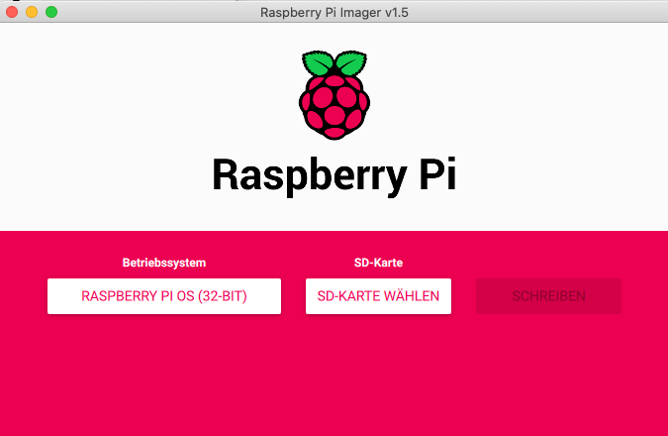
\includegraphics[width=0.7\linewidth]{abb/RaspberryPiImager}
	\caption{Raspberry Pi Imager}
	\label{fig:raspberrypiimager}
\end{figure}

Danach kann man die SD Karte in den Raspberry Pi einsetzen und ihn an einen Monitor, eine Tastatur, eine Maus anschließen und ihn schließlich mittels eines USB C-Netzkabels mit Spannung versorgen.
\subsection{Voreinstellungen}
Nach dem Start wird man durch ein kleines Wizard geführt, um diverse Einstellungen der Sprache und Lokalisierung, das Standard-Passwort des Nutzers pi, Bildschirm und Wlan zu ändern.
Falls es nach dem Wizard zu einem Fehler kommt oder das Tastatur-Layout nicht stimmt, kann man dies nach dem Neustart in den OS-Einstellungen ändern oder natürlich auch das Wizard beenden und die Einstellungen manuell durchführen.
\subsection{Update und Upgrade}
Nun wechseln wir im OS in das Terminal und geben den Befehl
\begin{lstlisting}[language=Bash]
sudo apt update  #die Quellen des Paketmanagers aktualisieren
sudo apt upgrade #installierte Pakete auf den aktuellen Stand setzen
#Gegebenenfalls muss man das Installieren der Pakete mit Y Enter bestätigen
\end{lstlisting}
\subsection{OPC UA Nutzer und Hostname anpassen}
Da es grundsätzlich nie ideal ist, auf einem bestehenden System bekannte Nutzer für den Zugriff von außen zu haben, benötigen wir einen neuen Benutzer. Außerdem wollen wir den hostname des Raspberry an unsere Bedürfnisse anpassen, da dieser für das Auffin-den von Geräten im Netzwerk nützlich ist.
Hostname ändern:
\begin{lstlisting}[language=Bash]
hostname #abrufen des aktuellen hostname
sudo hostname -b {neuerName} #ändern des hostname
hostname #prüfen, ob Änderung erfolgreich
sudo grep -lr „{alter hostname}” /etc/* #prüfen, ob der alte Host noch in anderen Konfiguratonsdateien verzeichnet ist

sudo nano /etc/{Dateiname}
#nach dem hostname suchen, ändern und mit ctrl x speichern, hier da-rauf achten, dass man keine Dateien ändern muss, wo in der Zeichenkette der hostname auftaucht(Bsp. raspi.list, hier findet man http.//archive.raspberrypi.org/debian/ das natürlich nicht ändern)
Außerdem muss man nicht die Keys von SSH ändern, diese erstellen wir gleich neu mit folgenden Befehlen

sudo rm /etc/ssh/ssh_host_* #alte Keys löschen
sudo dpkg-reconfigure openssh-server #neue Keys erstellen

sudo reboot #System-Neustart
\end{lstlisting}


Benutzer hinzufügen und Pi-Benutzer löschen:
\begin{lstlisting}[language=Bash]
#Nutzer hinzufügen
sudo adduser {USERNAME}
#Nutzer-Rechte hinzufügen, am wichtigsten ist sudo
sudo usermod -a -G adm,dialout,cdrom,sudo,ssh,audio,video,plugdev,games,users,input,netdev,gpio,i2c,spi {USERNAME}
#Testen, ob man sich mit dem neuen User als Superuser einloggen kann
sudo su – {USERNAME}
#den pi-Nutzer löschen
sudo pkill -u pi
#Nicht wundern, da wir im Desktop als PI-Nutzer eingeloggt sind und diesen gerade löschten, werden wir abgemeldet und gefragt, ob wir uns als {USERNAME} Nutzer einloggen wollen
\end{lstlisting}
\subsection{SSH}
Damit wir einen Fernzugriff auf den Raspberry bekommen, benötigen wir SSH. Dies können wir im Terminal mit folgenden Befehlen aktivieren.
\begin{lstlisting}[language=Bash]
sudo systemctl start ssh #ssh starten
sudo systemctl enable ssh #ssh Autostart nach dem boot Vorgang

systemctl status ssh #Status abfragen
systemctl is-enabled ssh #abfragen, ob Autostart aktiviert

ifconfig #damit sieht man die Einstellungen der Netzwerk Adpater, um sich für später die IP-Adresse (inet) des wlan0-Adpaters zu merken.
\end{lstlisting}

Nun können wir mit einem SSH Client auf den Raspberry zugreifen mit
\begin{lstlisting}[language=Bash]
 ssh {NUTZERNAME}@{IPADRESSE}
\end{lstlisting}
\subsection{Sicherheit}
Da davon ausgegangen wird, dass der Raspberry zunächst im lokalen Netz betrieben wird und wir während des Prototypings noch keine erhöhte Sicherheit benötigen, werden keine weiteren Sicherheitseinstellungen vorgenommen. Da aber später möglicherweise eine erhöhte Sicherheit benötigt wird, wird hiermit auf die offizielle Seite von \hyperref[https://www.raspberrypi.org/documentation/configuration/security.md 
]{www.raspberrypi.org} mit einer kleinen Guideline zu den Sicherheitseinstellungen, Firewall, SSH, Nutzer usw. verwiesen.
\clearpage
\section{Open62541 SDK am Raspberry kompilieren}\label{sec:open62541}
Die folgenden benötigten Pakete müssen auf dem Raspberry installiert werden. Einige Pakete sind bereits vorinstalliert.

\begin{lstlisting}[language=Bash]
sudo apt install git build-essential gcc pkg-config cmake python

# Nützliche Extra-Pakete
sudo apt install cmake-curses-gui # ccmake UI
sudo apt install libmbedtls-dev # Verschlüsselungs-Optionen
sudo apt install check libsubunit-dev # unit tests
sudo apt install python-sphinx graphviz #für Dokumentationen
sudo apt install python-sphinx-rtd-theme # Dokumentstyle-Erweiterung
\end{lstlisting}

Download des Source Codes
\begin{lstlisting}[language=Bash]
#Repository Clone
git clone https://github.com/open62541/open62541.git ~/open62541
#Gehen in den Ordner
cd ~/open62541 #Submodule Laden
git submodule update --init --recursive
\end{lstlisting}

Kompilierung vorbereiten mit CCmake
\begin{lstlisting}[language=Bash]
#Pfad erstellen und in Pfad gehen
mkdir ~/open62541/build && cd ~/open62541/build
#Öffne ccmake UI aus den Informationen im unteren Pfad
ccmake ..
\end{lstlisting}

Nun öffnet sich die UI. In dieser betätigen wir zunächst die Taste „c“, um die Konfigurations-Seite zu öffnen. Wie in \autoref{fig:buildopen62541} zu sehen, ändern wir den CMAKE\_BUILD\_TYPE gegen RelWithDebInfo (Release Version mit Debug-Informationen), das 
CMAKE\_INSTALL\_PREFIX gegen den Installationspfad und den UA\_NAMESPACE\_ZERO gegen FULL (Volle „namespace zero“-Erstellung von den offiziellen XML-Definitionen.) . Nachdem wir fertig sind, beenden wir die Einstellungen mit der Taste „c“ und erstellen ein make file mit der Taste „g“.
Danach bauen wir den Code mit dem Befehl
\begin{lstlisting}[language=Bash]
make -j #das kann einige Zeit dauern
make install #den Build ins vorher gesetzte Installationsverzeichnis verschieben
\end{lstlisting}
  
\begin{figure}[H]
	\centering
	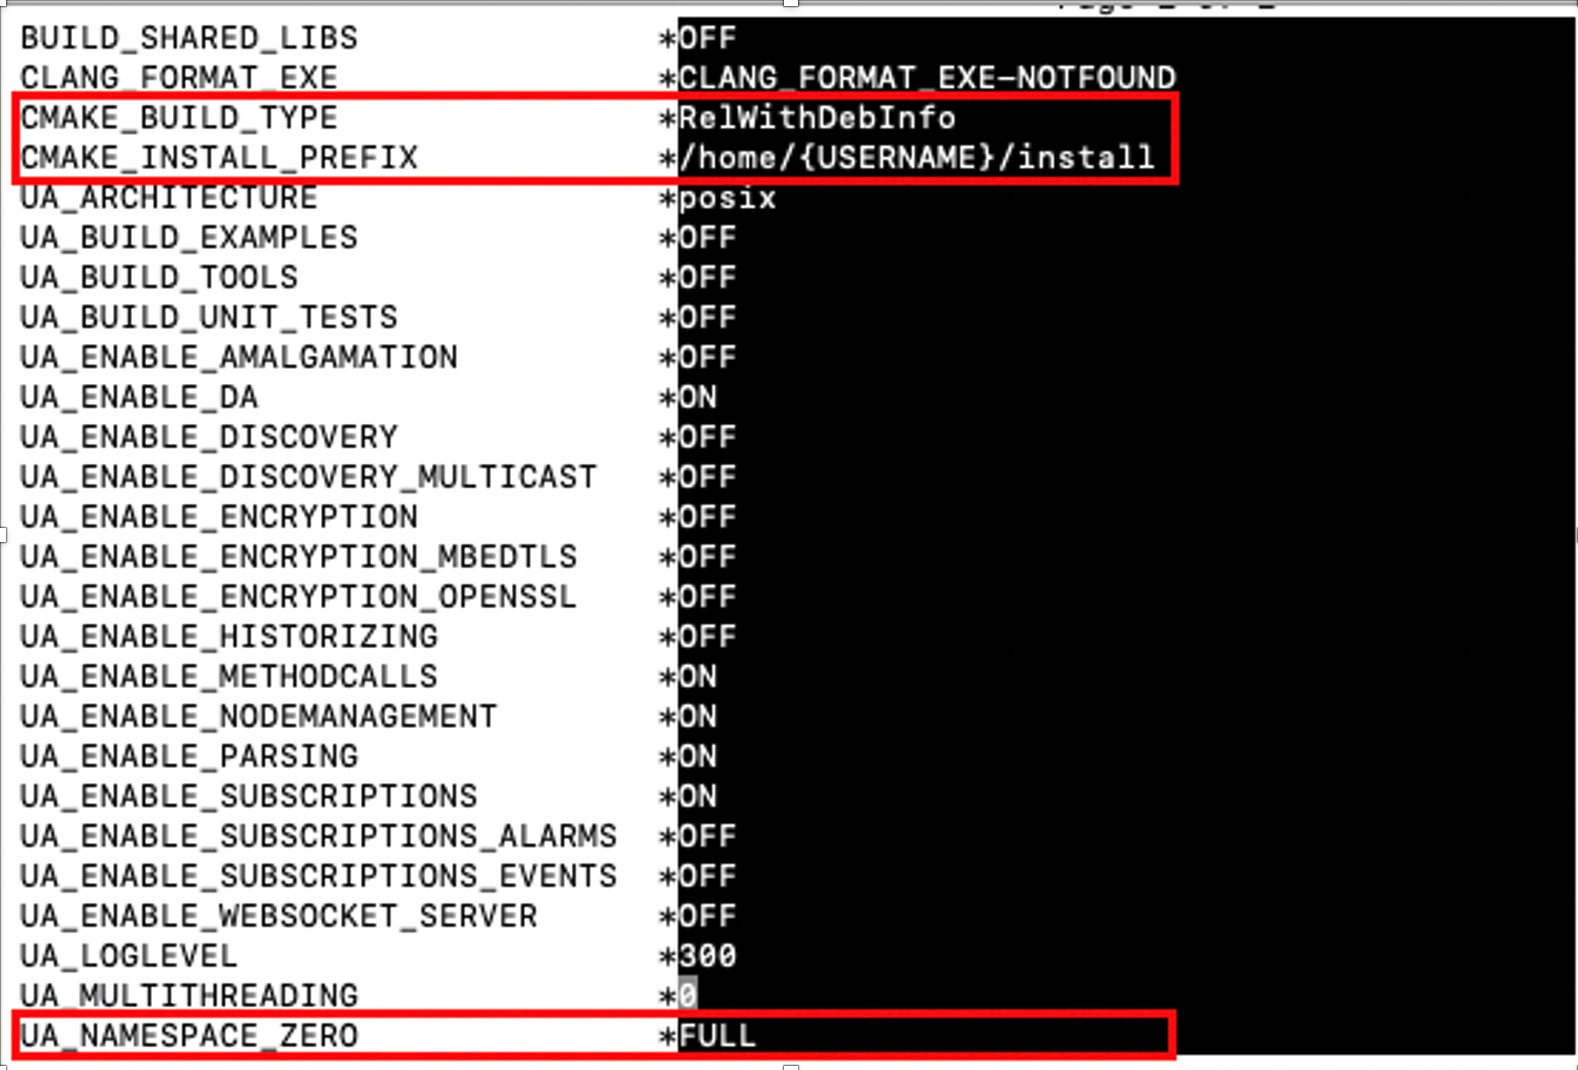
\includegraphics[width=0.6\linewidth]{abb/Build_Open62541}
	\caption{ccmake-Einstellungen}
	\label{fig:buildopen62541}
\end{figure}

Anmerkung:
Entgegen der Empfehlung kann es gerade am Anfang Sinnvollsein nicht den NamepsaceFull zu benutzen, sondern Reduced. Dies spart gerade am Anfang beim Ausprobieren viel Zeit beim Kompilieren, wenn man auf einige vordefinierte Typen verzichten kann.
Ein Überblick der beinhalteten Typen vom Namespace Reduced findet man hier:
https://github.com/open62541/open62541/blob/master/tools/schema/Opc.Ua.NodeSet2.Reduced.xml

\subsection{Erster Server mit OPC UA als Test}
Nun wollen testen, ob alles funktioniert. Deshalb kopieren wir uns ein Beispiel eines Ser-vers und erstellen daraus einen lauffähigen Server auf dem Raspberry
\begin{lstlisting}[language=Bash]
mkdir ~/firstTest-Server
cp ~/open62541/examples/tutorial_server_firststeps.c ~/firstTestServer/firstTestServer.c
cd ~/firstTestServer/

#Bauen des TestServers
gcc -std=c99 -flto=1 -I$HOME/install/include -L$HOME/install/lib firstTestServer.c -lopen62541 -lmbedtls -lmbedx509 -lmbedcrypto -o firstTestServer
\end{lstlisting}
Dies kann über eine Stunde dauern.
Was wurde im gcc-Befehl gemacht:
\begin{itemize}
	\item std=c99 gcc benutzt den C99-Kompilierer
	\item flto=1 limitiert die parallel ablaufenden Linking-Jobs auf 1
	\item -I{PFAD} fügt den vorhin gebauten Include-Pfad hinzu
	\item -L{PFAD} fügt den vorhin gebauten Library-Pfad hinzu
	\item \$Home Verweis auf das home-Verzeichnis des aktuellen Nutzers ähnlich wie ~/ nur universeller einsetzbar.
	\item firstTest-Server.c  C-Datei, die gebaut werden soll
	\item -lopen62541 open62541 Library
	\item -lmbedtls -lmbedx509 -lmbedcrypto für Kryptographie
	\item -o firstTestServer Ausgabe-Datei
\end{itemize}

\subsection{Test-Server mit Client verbinden}
Nun können wir den Server testen, indem wir die gerade erstellte Datei ausführen
\begin{lstlisting}[language=Bash]
./firstTestServer
\end{lstlisting}
\begin{figure}[H]
	\centering
	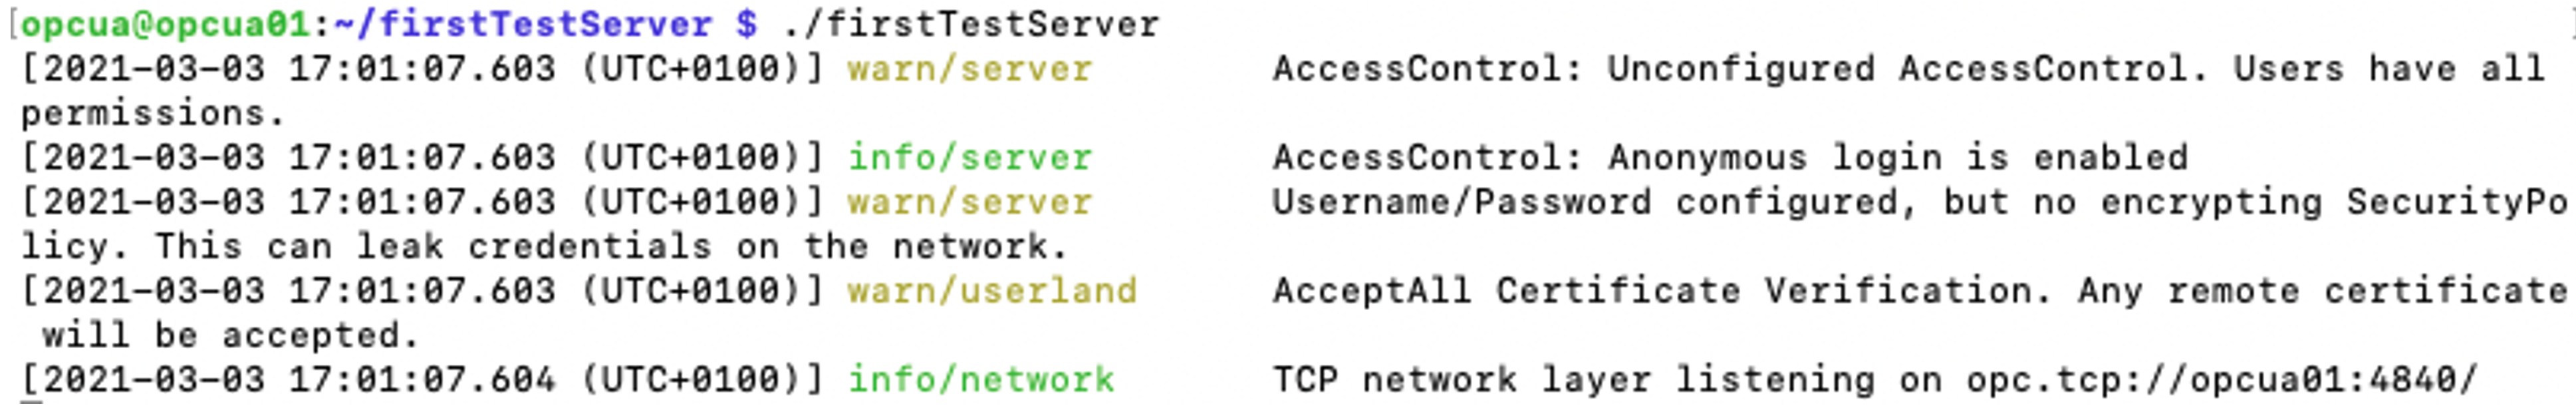
\includegraphics[width=1\linewidth]{abb/TerminaNachServerStart}
	\caption{Terminal-Ausgabe nach dem Start des OPC UA-Servers}
	\label{fig:terminanachserverstart}
\end{figure}


In \autoref{fig:terminanachserverstart} sieht man den Server, der sich gestartet hat sowie die Adresse mit Port, unter der er erreichbar ist. Nun starten wir auf unserem Computer die Software UA Expert und fügen, wie in \autoref{fig:uaexpertclient} zu sehen ist, den gerade gestarteten Server hinzu. 

\begin{figure}[H]
	\centering
	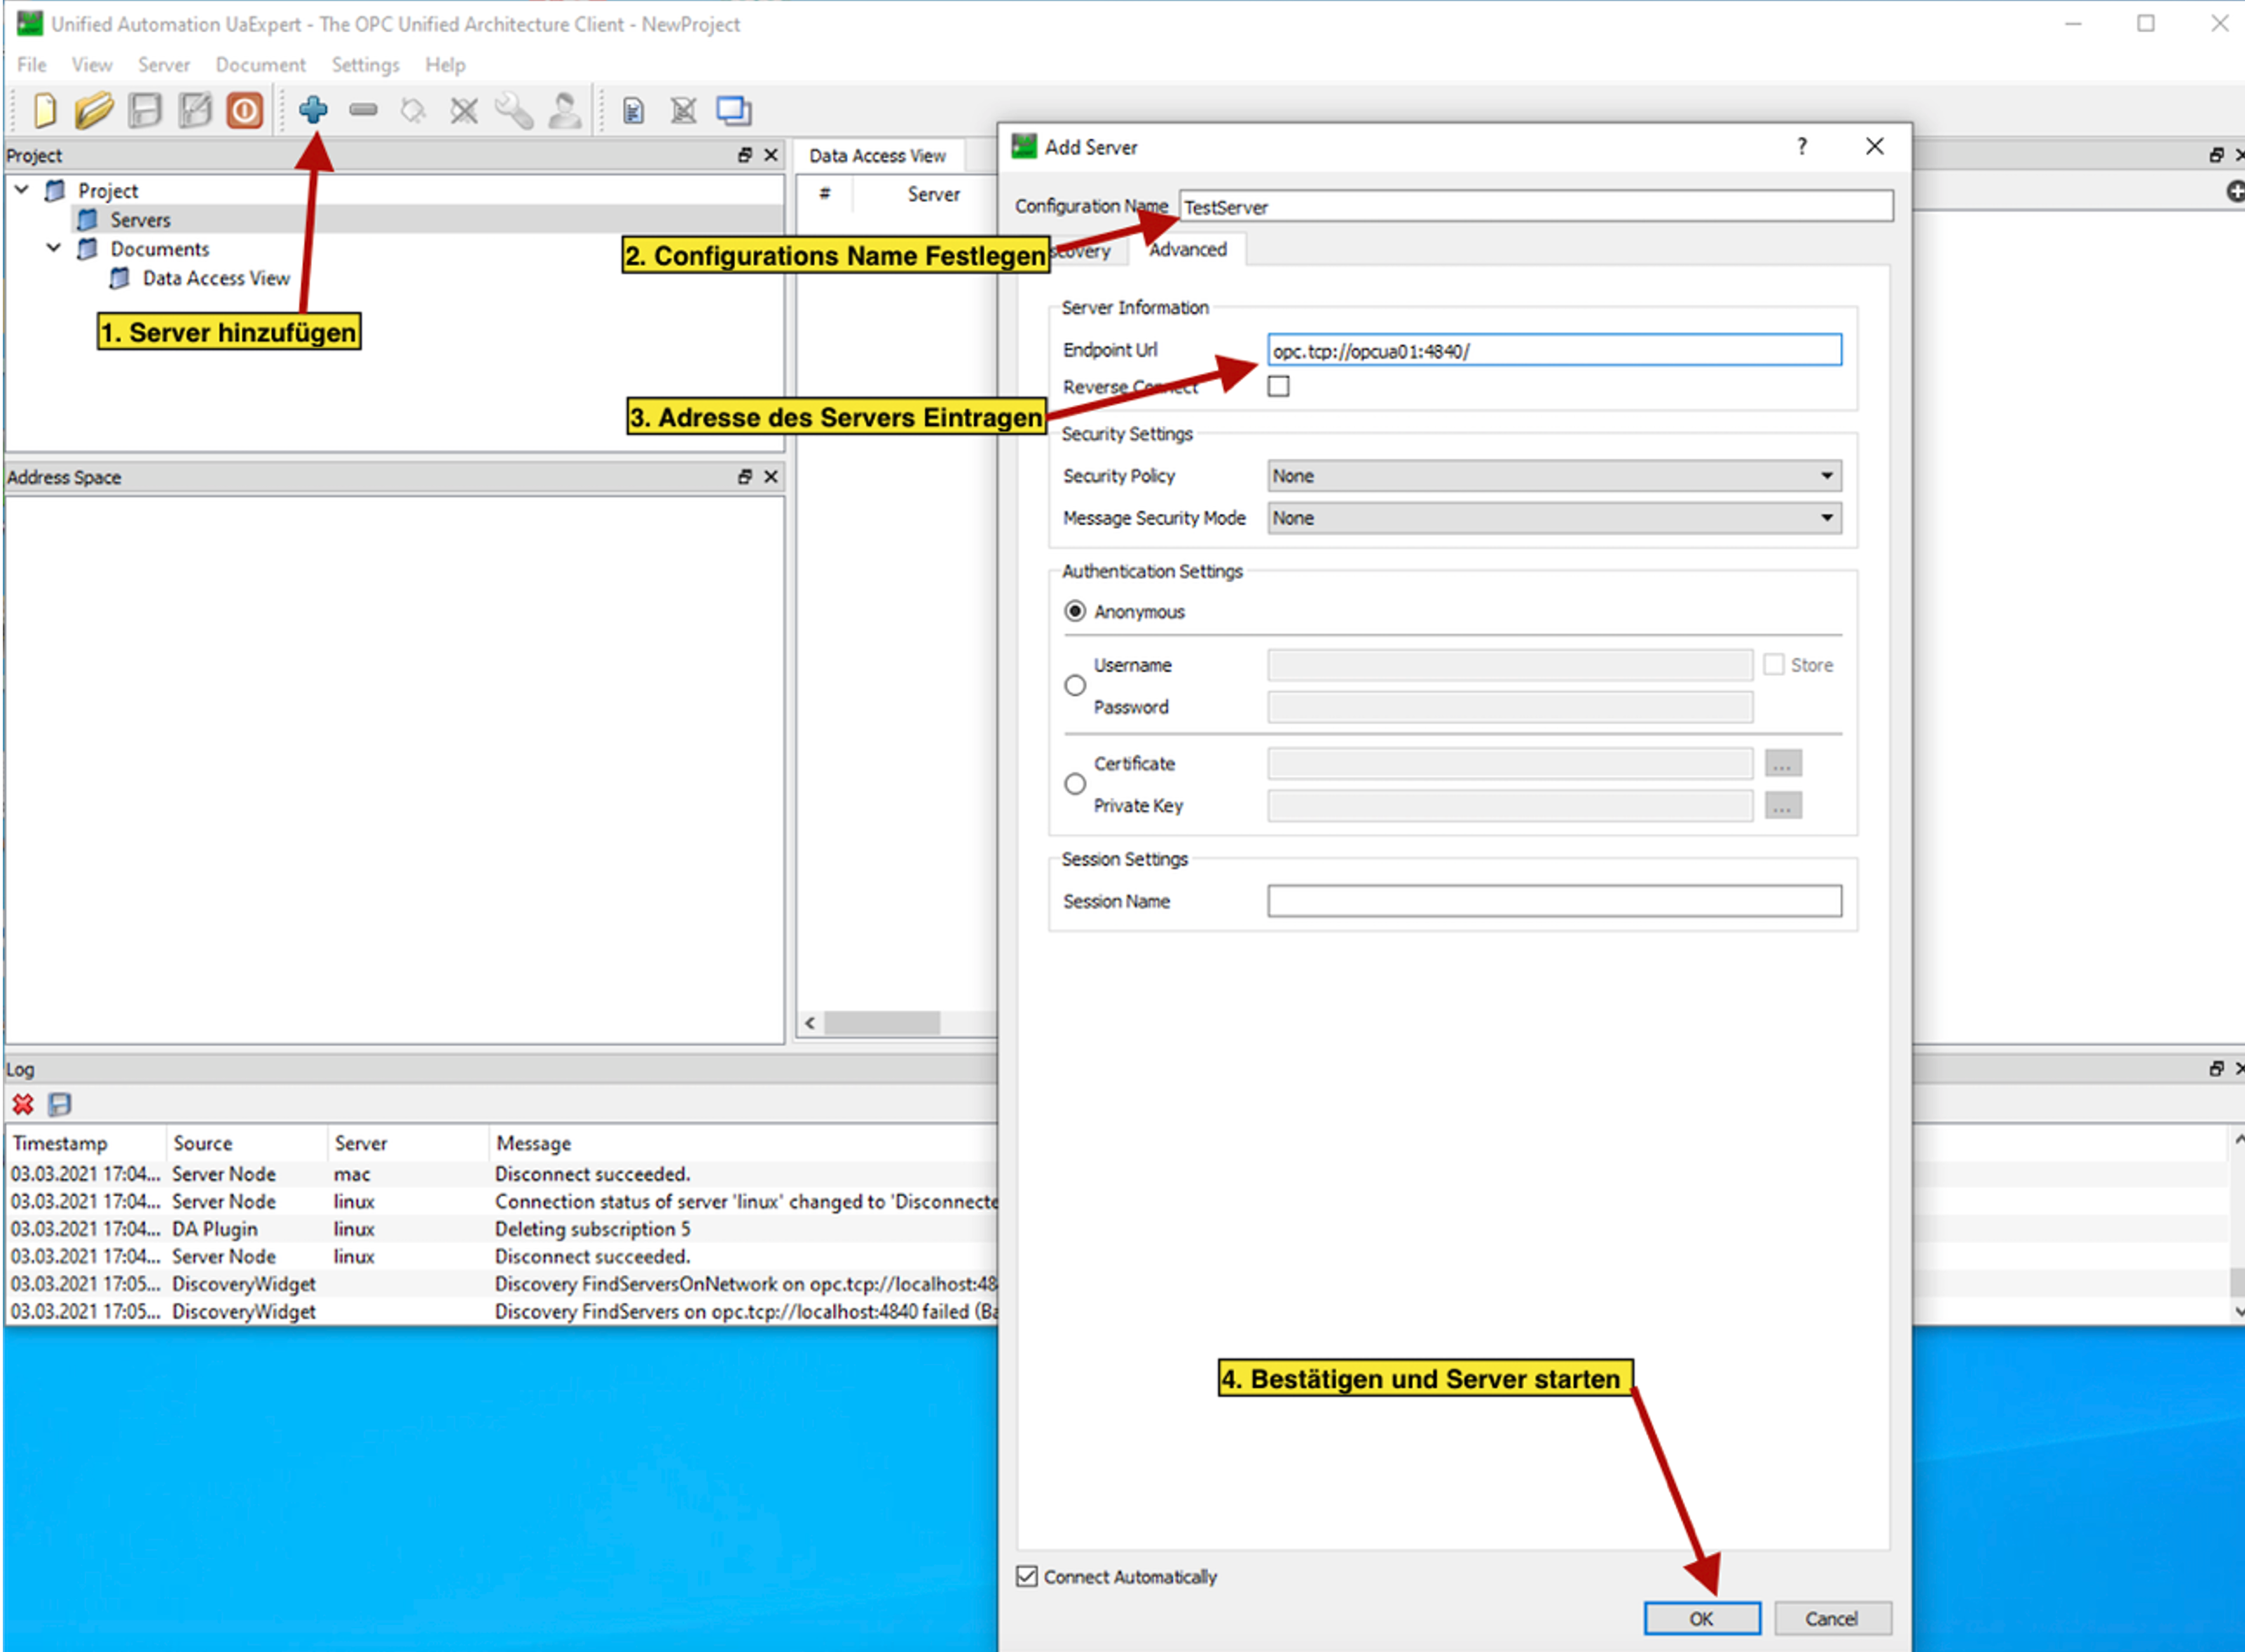
\includegraphics[width=1\linewidth]{abb/UA_ExpertClient}
	\caption{Erster Start UA Expert}
	\label{fig:uaexpertclient}
\end{figure}

Danach sieht man in  die Datenstruktur des erstellten Test-Servers wie in \autoref{fig:uaexpertstrukt}

\begin{figure}[H]
	\centering
	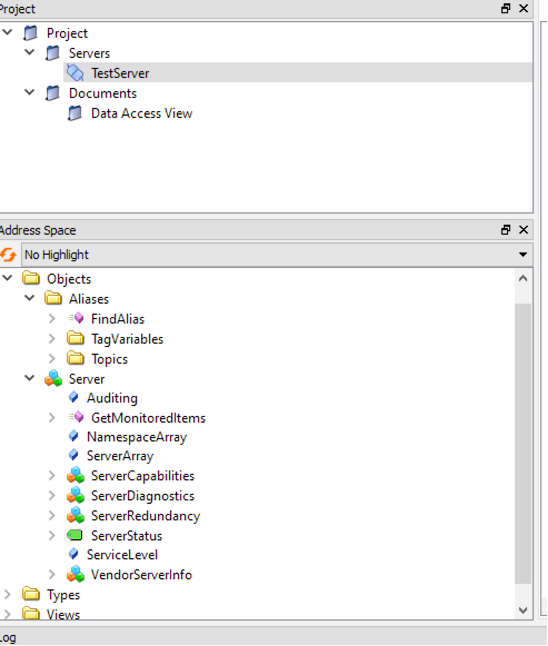
\includegraphics[width=0.6\linewidth]{abb/UA_Expert_Strukt}
	\caption{Daten-Struktur Test-Server in UA Expert}
	\label{fig:uaexpertstrukt}
\end{figure}
\clearpage
\section{Informationsmodellierung eines OPC UA-Servers}
Nachdem jetzt die Grundlagen geschaffen sind, einen lauffähigen OPC UA-Server zu erstellen, wird in diesem Kapitel erklärt, wie man mit Hilfe des FreeOpcUa Modeler ein UANodeSet.xml für seine Server-Struktur erstellt. Dies wird im nächsten Kapitel benö-tigt, um einen Server mit einem eigenen Nodeset zu bauen. Eine detaillierte Erklärung zu Informationsmodellen und auch noch andere Wege zur Erstellung seiner Informationsmodelle findet man unter \hyperref[https://opcua.rocks/]{https://opcua.rocks/} 

\subsection{FreeOpcUa Modeler}
Das Programm können wir entweder direkt auf dem Raspberry installieren und ausführen oder auch auf dem Projekt-Rechner.
Nachdem wir diesen gestartet haben, läuft im Hintergrund auch schon automatisch ein OPC UA-Server, mit dem man sich verbinden kann. Dieser Server läuft auf dem Open Source Projekt FreeOPC UA. Es soll auch möglich sein, hier direkt einen open62541-Server anzusprechen. Da wir dies in unserem Beispiel nicht benötigten, wurde das nicht getestet.
Ein Blick nach dem Start im Terminal zeigt auch hier die generierte opc-Adresse mit Port, wie in \autoref{fig:freeopcua} zu sehen. 0.0.0.0 bedeutet, dass dieser am local Host erreichbar ist. Um sich also mit ihm über einen anderen Rechner im Netzwerk zu verbinden, wird die IP-Adresse des Netzwerk-Adapters benötigt!
\begin{figure}[H]
	\centering
	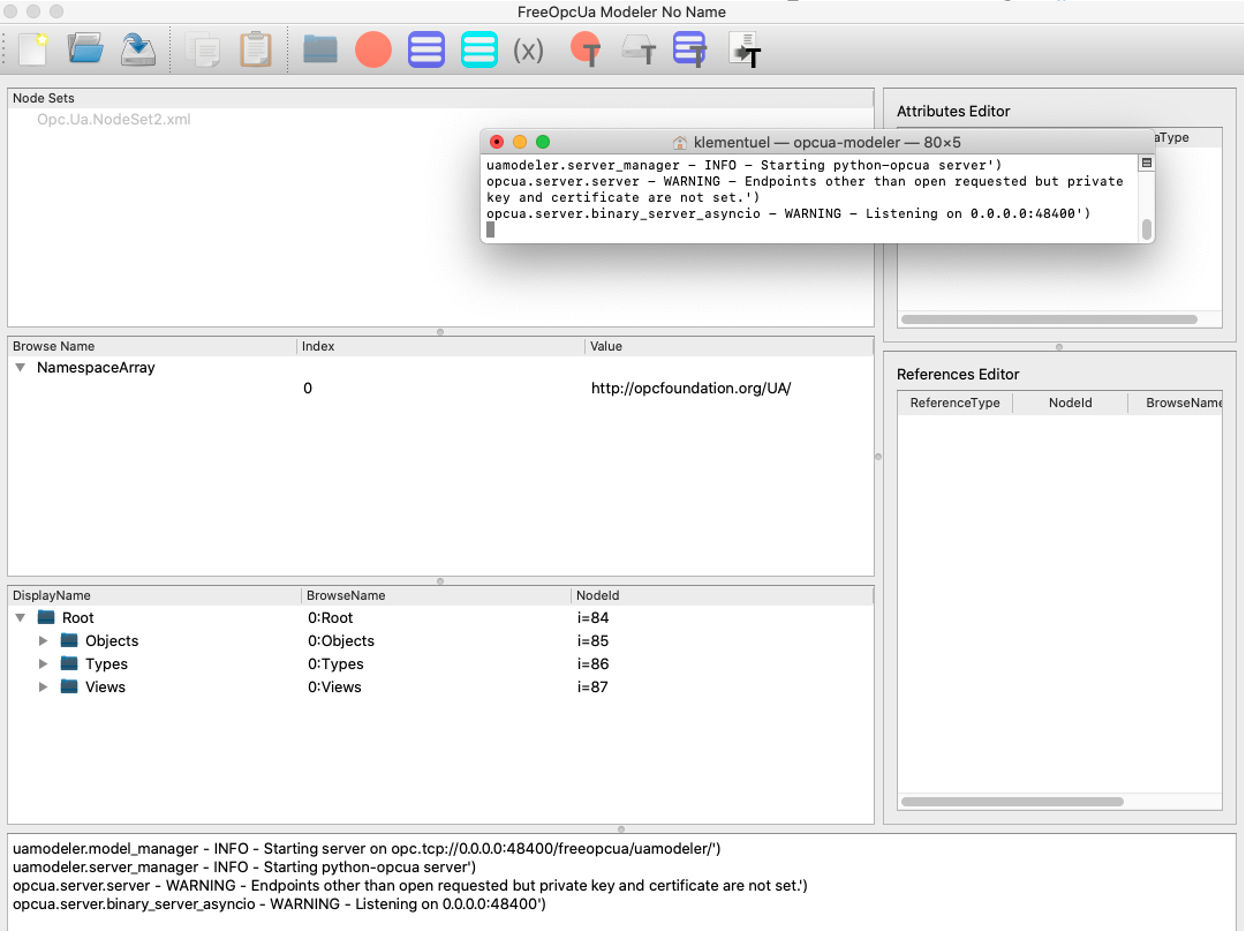
\includegraphics[width=1\linewidth]{abb/FreeOPCUA}
	\caption{Start FreeOpcUa Modeler}
	\label{fig:freeopcua}
\end{figure}
Nun beginnen wir mit der Modellierung eines einfachen Beispiels:
Wir haben einen Motor, der über das Datenmodell ansteuerbar sein und seinen Status anzeigen soll. Es kann auch sein, dass noch ein Motor hinzukommt.
Als erstes benötigen wir einen Namespace, wo wir diese Typen, Objekte später zuordnen. Wie in \autoref{fig:addnamespace} zu sehen, wurde der Namespace 1 mit http.//motoren.test/UA/ er-stellt.
\begin{figure}[H]
	\centering
	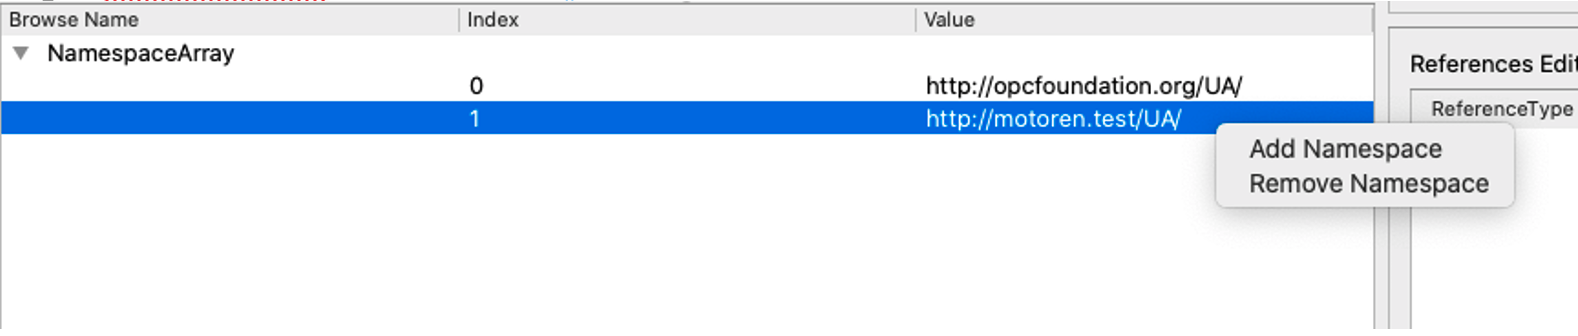
\includegraphics[width=1\linewidth]{abb/AddNamespace}
	\caption{Namespace erstellen}
	\label{fig:addnamespace}
\end{figure}
Da es also sein kann, dass wir mehrere Motoren benötigen, erstellen wir als Erstes einen Motor-Typ, der ein Objekt eines Motors darstellt und beliebig oft als Objekt wiederverwendet werden kann. In \autoref{fig:objecttypanlegen} ist der Ablauf einer Objekt-Typ-Erstellung zu sehen.
\begin{figure}[H]
	\centering
	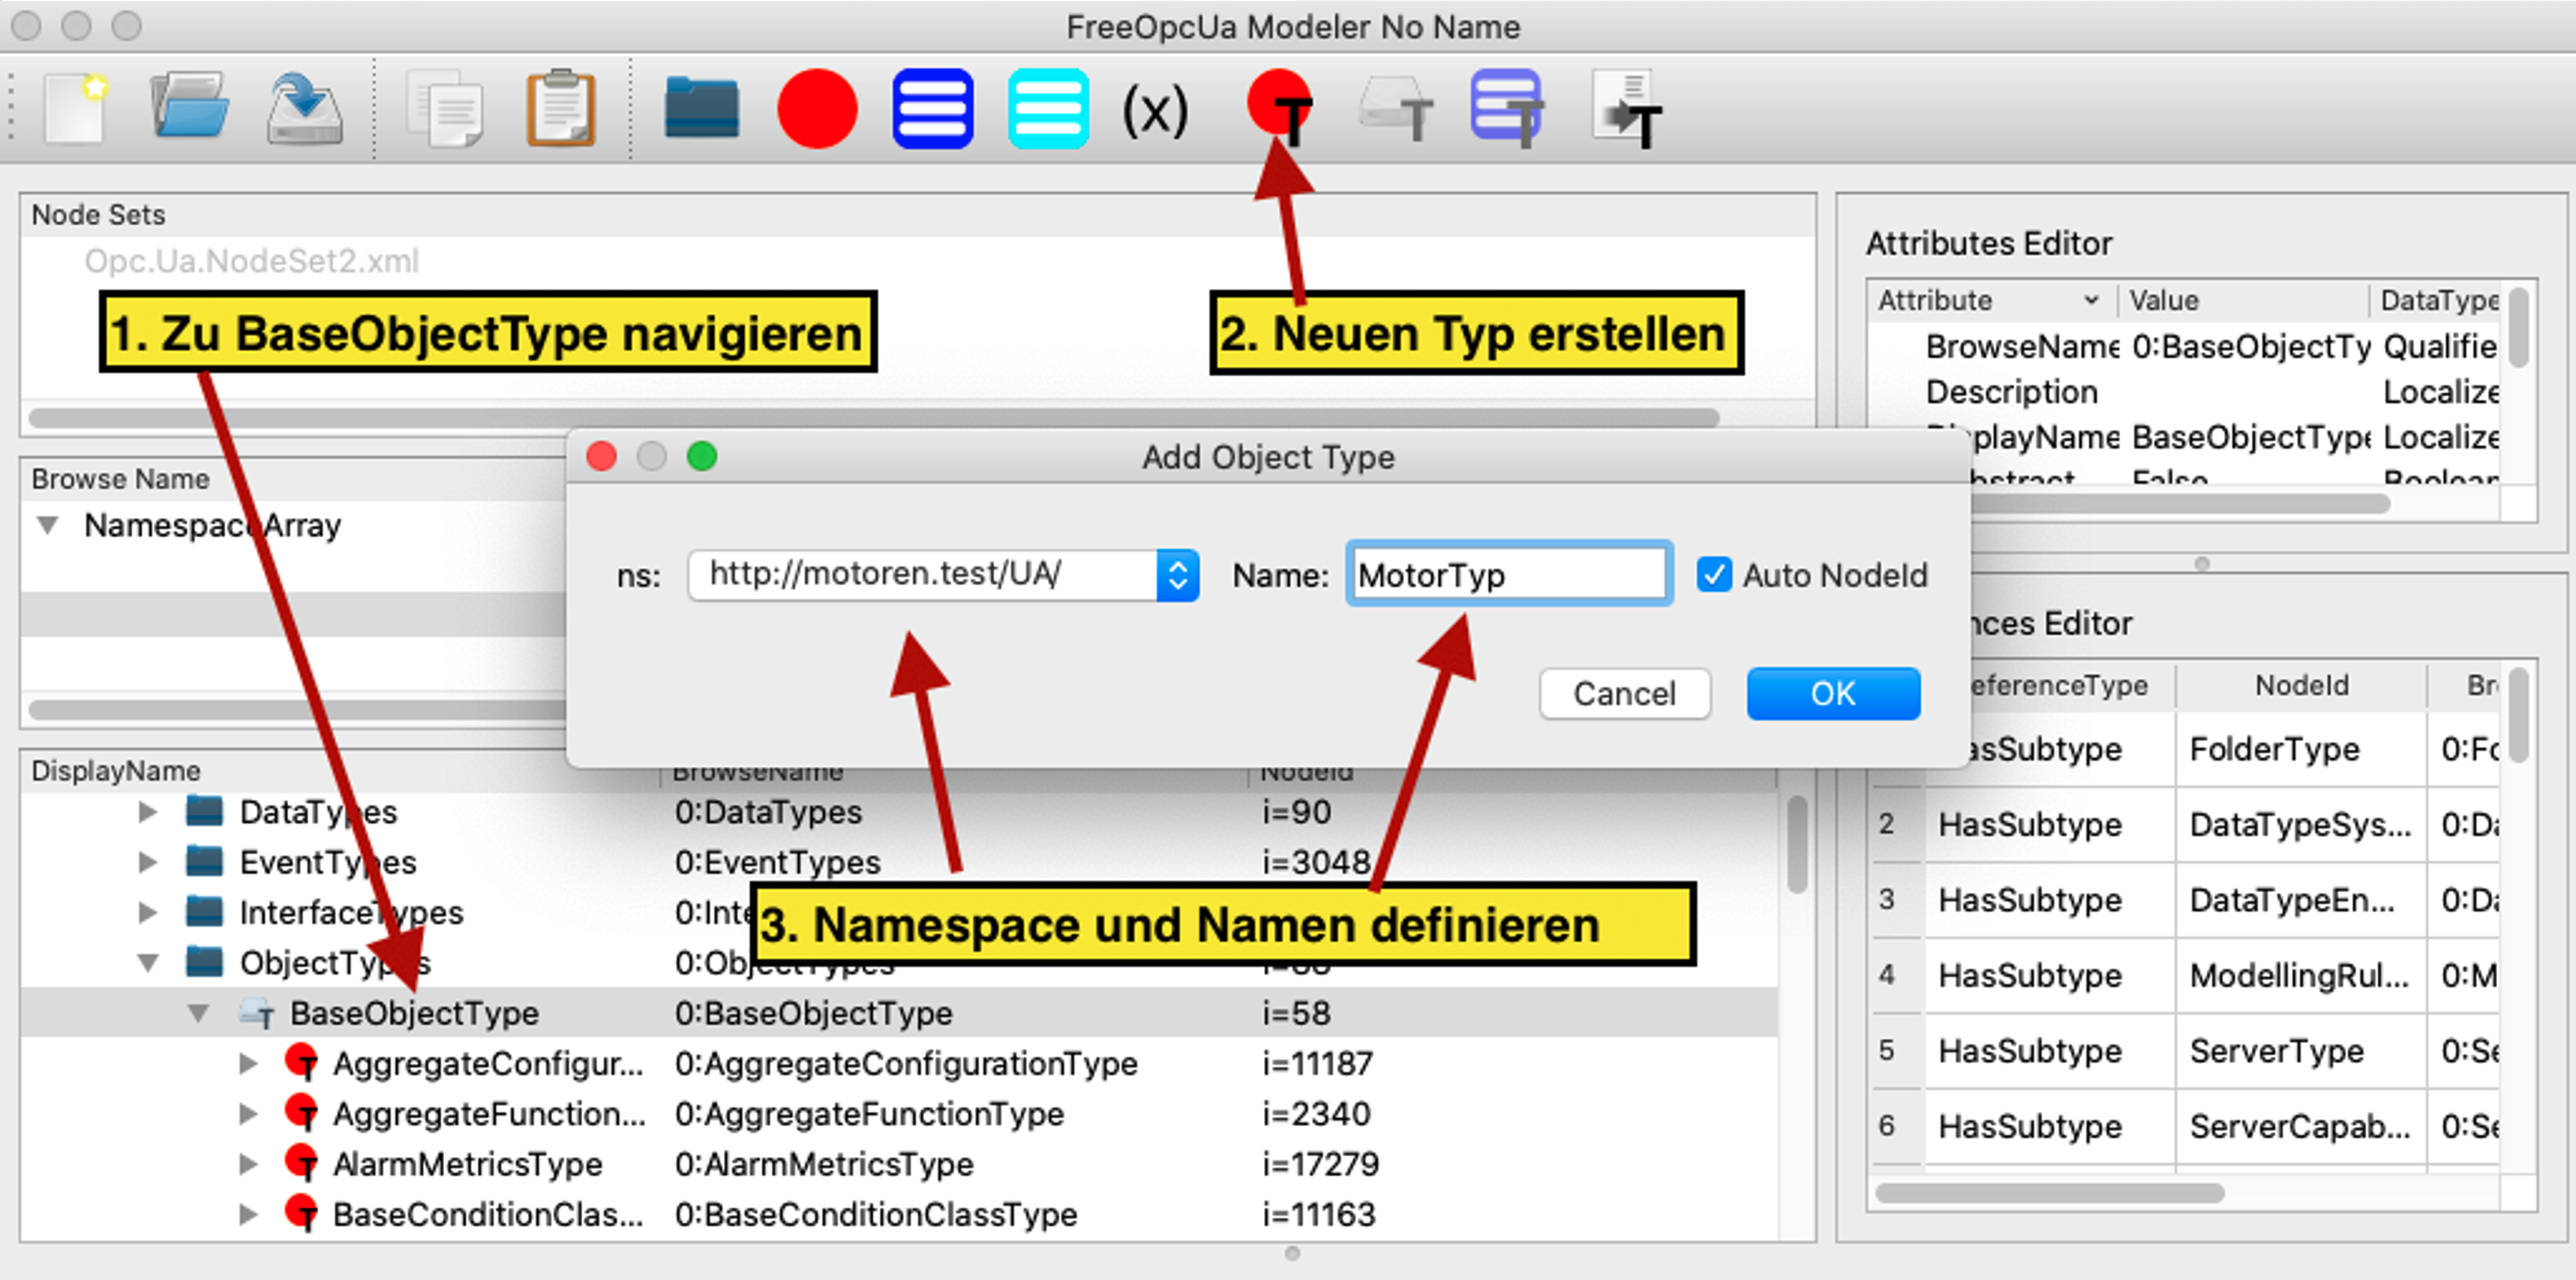
\includegraphics[width=1\linewidth]{abb/ObjectTypAnlegen}
	\caption{Objekt-Typ anlegen}
	\label{fig:objecttypanlegen}
\end{figure}
Nun werden dem Objekt-Typ die nötigen Informationen gegeben.
Im Beispiel wurden 3 Variablen erstellt, die der Nutzer nur lesen kann (Speed, Running, Direction) und 2 Methoden Control mit Eingangs- und Ausgangs-Variablen und Emergency Stop ohne Variablen, wie in \autoref{fig:erweitertmotorty} zu sehen.
\begin{figure}[H]
	\centering
	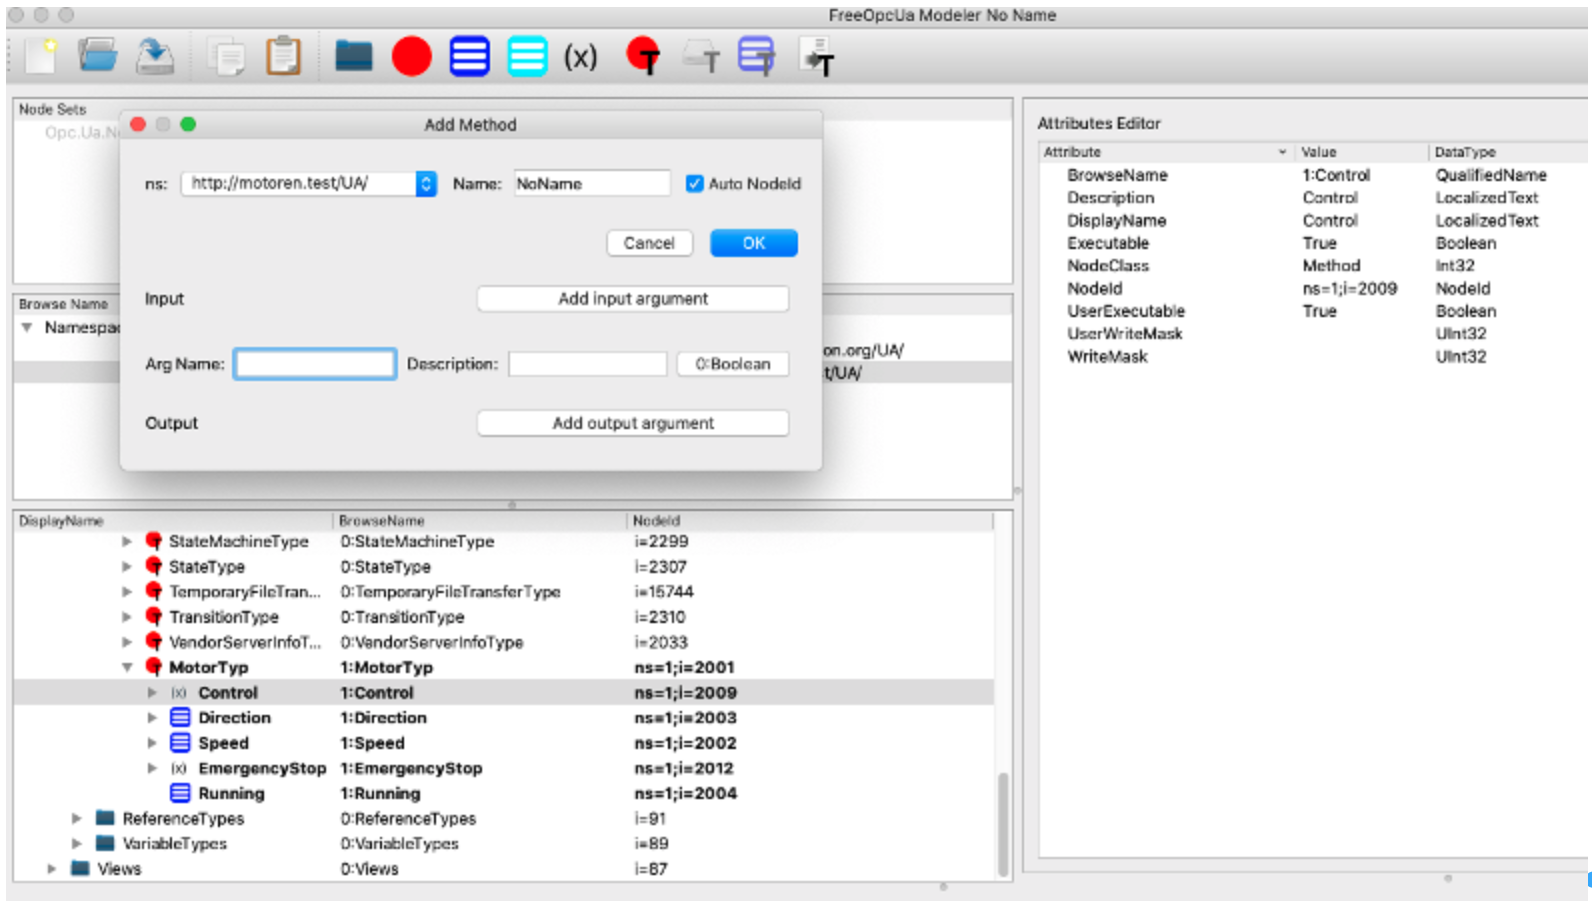
\includegraphics[width=1\linewidth]{abb/ERweitertMotorTy}
	\caption{Erweitern der Informationen des Motor-Typs}
	\label{fig:erweitertmotorty}
\end{figure}
Im nächsten Schritt wird aus dem erstellten Typ ein Objekt erstellt (\autoref{fig:addobject}).
\begin{figure}[H]
	\centering
	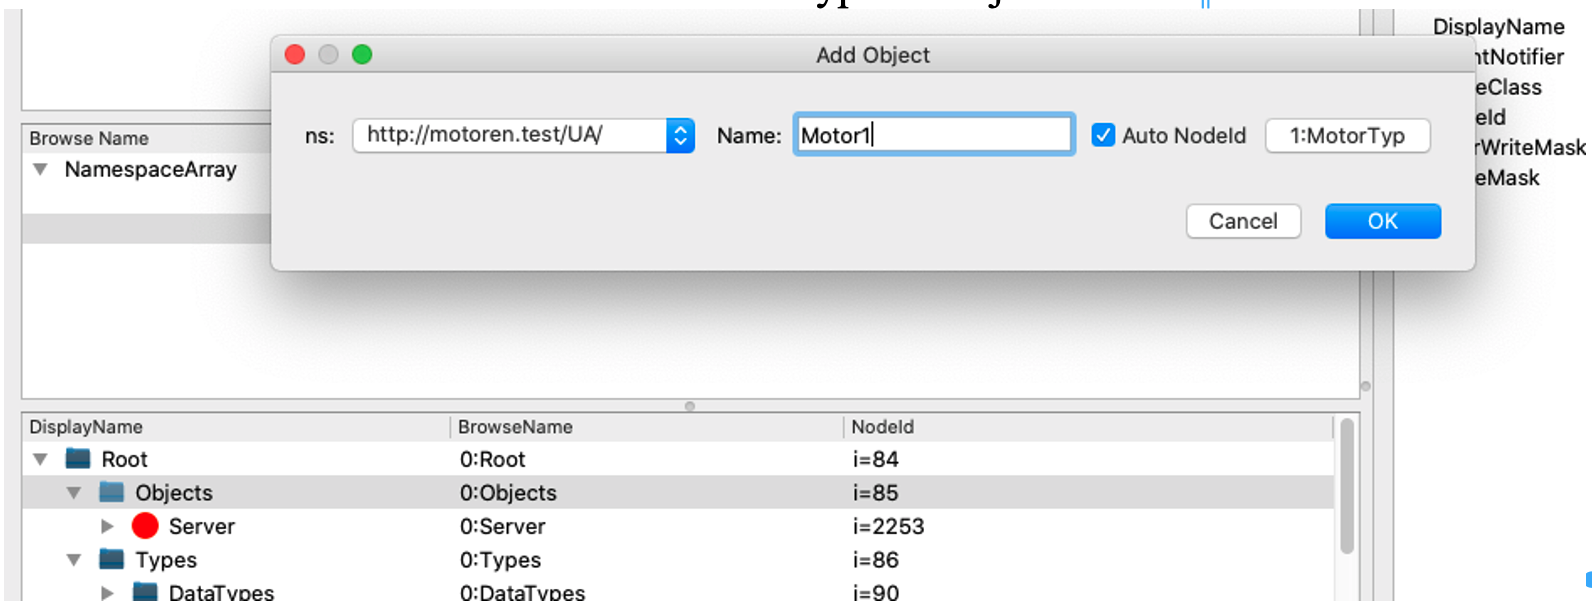
\includegraphics[width=1\linewidth]{abb/AddObject}
	\caption{Erstellen eines Objekts aus einem Objekt-Typ}
	\label{fig:addobject}
\end{figure}
Und schon kann im UA Expert Client die Struktur validiert werden, wie \autoref{fig:callmethodeuaexpert} zeigt.
\begin{figure}[H]
	\centering
	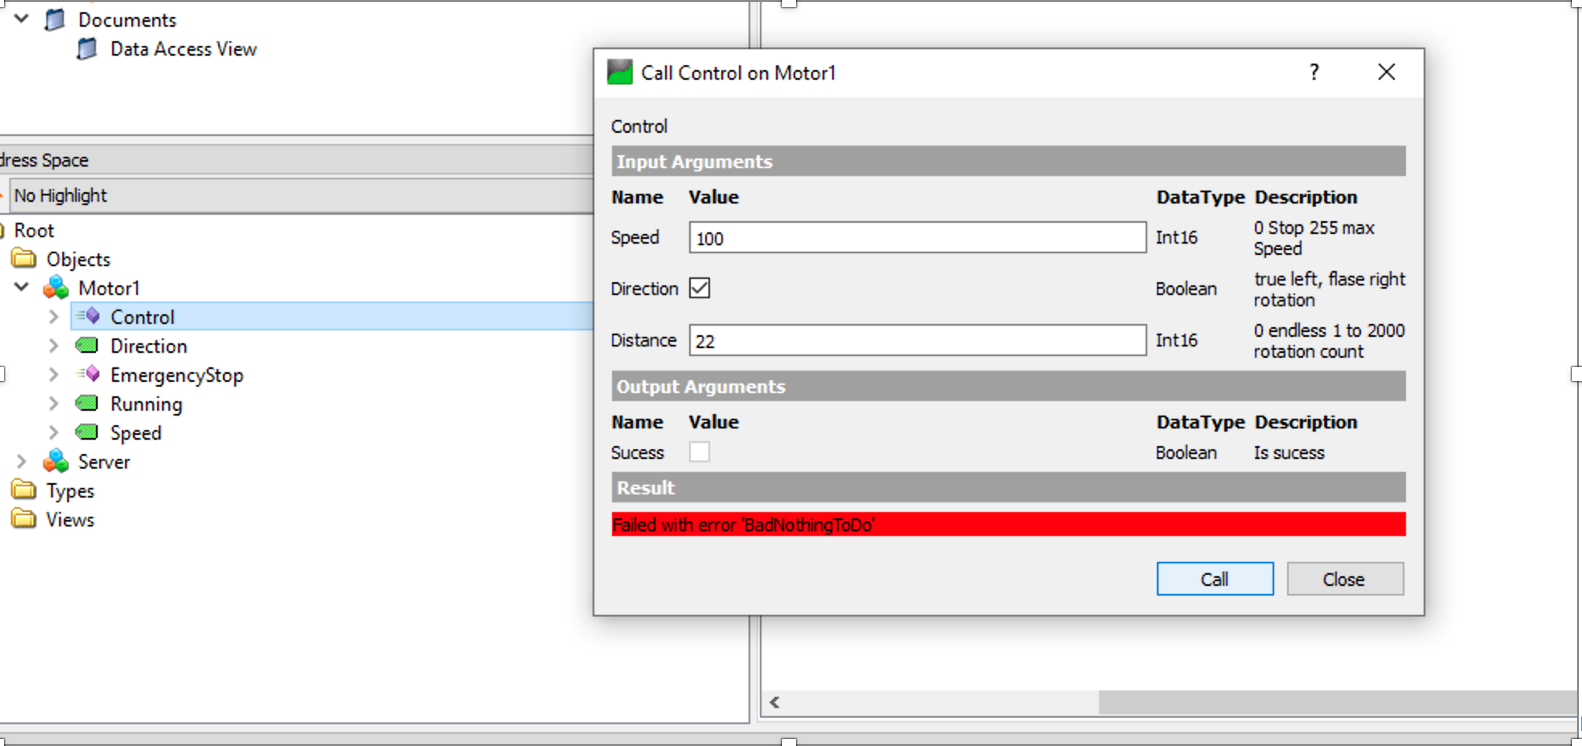
\includegraphics[width=1\linewidth]{abb/CallMethodeUAExpert}
	\caption{UA Expert Aufruf einer Methode}
	\label{fig:callmethodeuaexpert}
\end{figure}
Natürlich führt der Aufruf einer Methode, wie auch zu sehen ist, noch zu einem Fehler, da noch keine Logik in den Methoden steckt.
Nun wird das Projekt noch abgespeichert, wodurch sich auch das benötigte UANodeSet File als XML Datei generiert.
(\autoref{fig:nodesetxml})
\begin{figure}[H]
	\centering
	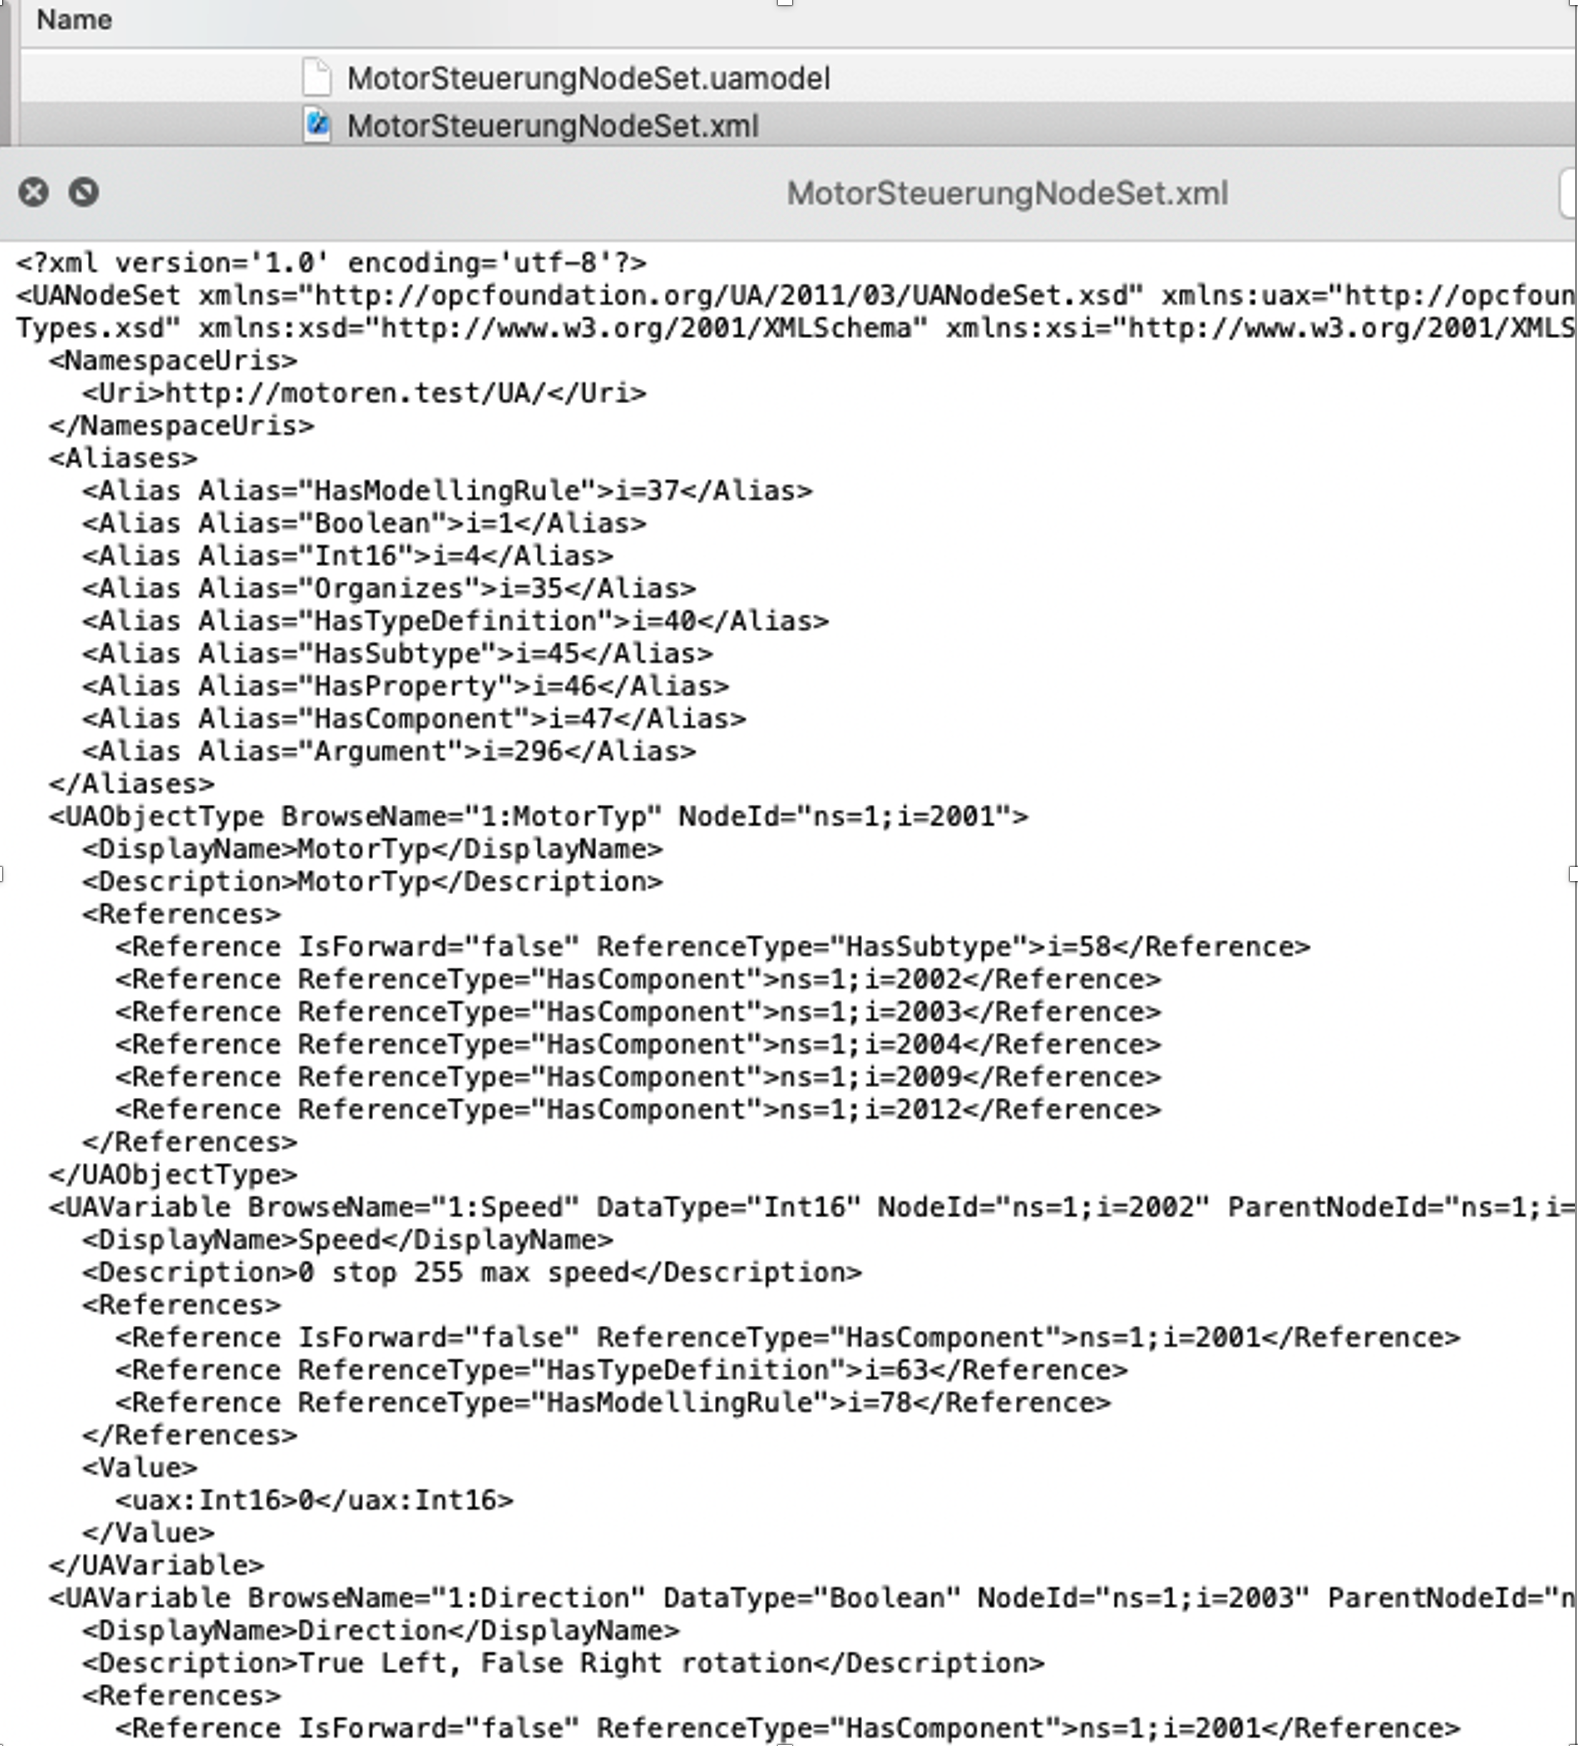
\includegraphics[width=0.8\linewidth]{abb/NodesetXML}
	\caption{Auszug aus der gespeicherten xml}
	\label{fig:nodesetxml}
\end{figure}

Anmerkung: Es ist nicht nötig, hier schon Objekte anzulegen, denn diese kann man auch später erstellen. Wenn man allerdings schon weiß, was man braucht, ist es nützlich, diese gleich zu modellieren. Des Weiteren ist es ebenso möglich, aus einem Typ Objekt-Varianten zu erstellen, wenn man z.B. danach noch Variablen hinzufügt, um einzelne Objekte zu spezialisieren.

\clearpage
\section{Aus einem UANodeSet.xml den Source-Code erstellen}
Im Grunde ist dies recht einfach, da im Git Reprository von open62541 ein python skript hinterlegt ist, das die ganze Arbeit erledigt. Dies kann man also auch direkt am Raspberry erledigen oder auch auf seinem Projekt-Computer.
Hierfür muss nun das Skript mit folgenden Zusätzen ausgeführt werden.
\begin{lstlisting}[language=Bash]
python ~/open62541/tools/nodeset_compiler/nodeset_compiler.py 
--types-array=UA_TYPES --existing ~/open62541/deps/ua-nodeset/Schema/Opc.Ua.NodeSet2.xml --xml MotorSteuerungNodeSet.xml MotorSteuerung
\end{lstlisting}
Kurze Erklärung zu den einzelnen Zusätzen
\begin{lstlisting}[language=Bash]
# python skript, das ausgeführt werden muss
python ~/open62541/tools/nodeset_compiler/nodeset_compiler.py
# als was sollen die Typen exportiert werden
--types-array=UA_TYPES
# auf welchem Schema baut das Ganze auf
--existing ~/open62541/deps/ua-nodeset/Schema/Opc.Ua.NodeSet2.xml
#Pfad zum erstellten NodeSet2.xml
--xml MotorSteuerungNodeSet.xml
#Ausgabe-Name, aus diesem werden dann die benötigte c- und h-Datei erstellt
MotorSteuerung
\end{lstlisting}
Wenn das Ganze erfolgreich war, sollte es wie in  aussehen. Im oberen Teil sieht man die Ausgabe des Skripts, im unteren Teil die im Ordner erstellten c- und h-Dateien.
\begin{figure}[H]
	\centering
	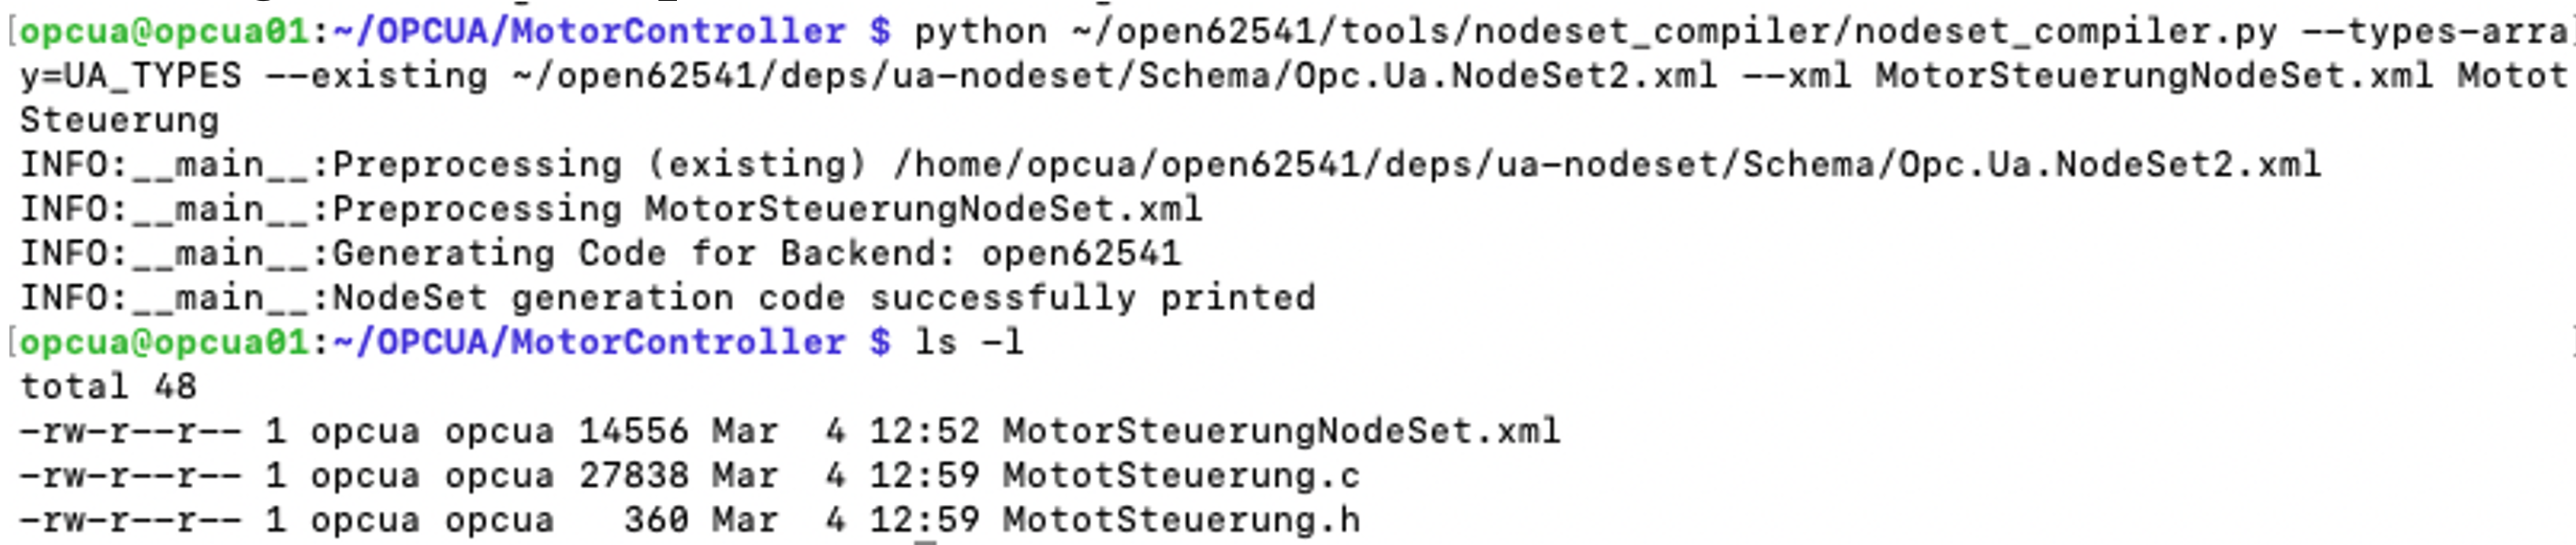
\includegraphics[width=1\linewidth]{abb/ErfolgSource}
	\caption{Erfolgreiche Erstellung des Source Codes}
	\label{fig:erfolgsource}
\end{figure}
\clearpage
\section{Erstellen der Main-Methode und erster Server -Test}
In dem vorhergehenden Kapitel wurde der Source Code aus einem Informationsmodell erstellt. Nun wollen wir das Ganze durch das Erstellen einer Main-Methode ergänzen, die als Startpunkt für den Server dient. Dazu erstellen wir in einem beliebigen Editor mit fol-gendem Inhalt eine main.c-Datei und speichern diese bei unserem Source Code ab.
\begin{lstlisting}[language=Bash]
#include <open62541/plugin/log_stdout.h>
#include <open62541/server.h>
#include <open62541/server_config_default.h>
#include <signal.h>
#include <stdlib.h>
#include "MotorSteuerung.h"

UA_Boolean running = true;


static void stopHandler(int sign) {
	UA_LOG_INFO(UA_Log_Stdout, UA_LOGCATEGORY_SERVER, "received ctrl-c");
	running = false;
}

int main(int argc, char** argv) {
	signal(SIGINT, stopHandler);
	signal(SIGTERM, stopHandler);
	
	UA_Server *server = UA_Server_new();
	UA_ServerConfig_setDefault(UA_Server_getConfig(server));
	UA_StatusCode retval;
	/* create nodes from nodeset */
	if(MotorSteuerung(server) != UA_STATUSCODE_GOOD) {
		UA_LOG_ERROR(UA_Log_Stdout, UA_LOGCATEGORY_SERVER,
		"Could not add the MotorSteuerung nodeset. "
		"Check previous output for any error.");
		retval = UA_STATUSCODE_BADUNEXPECTEDERROR;
	} else {
		// Do some additional stuff with the nodes
		// this will just get the namespace index,
		//since it is already added to the server
		UA_UInt16 nsIdx = UA_Server_addNamespace(server, "http://helloWorld.com/UA/");
		// UA_MOTOR1_RUNNING_BOOL = 2010
		UA_NodeId testInstanceId = UA_NODEID_NUMERIC(nsIdx, 2010);
		UA_LOG_INFO(UA_Log_Stdout, UA_LOGCATEGORY_SERVER,
		"Motor1 Bool Running is in ns=%d;id=%d",
		testInstanceId.namespaceIndex, testInstanceId.identifier.numeric);
		retval = UA_Server_run(server, &running);
	}
	UA_Server_delete(server);
	return retval == UA_STATUSCODE_GOOD ? EXIT_SUCCESS : EXIT_FAILURE;
\end{lstlisting}
	Wie man erkennen kann, wird in der Main-Methode ein Server-Objekt mit den Standard- Einstellungen erstellt. Die Variable retval dient dazu, nach dem Beenden den Staus-Code des Servers zurückzugeben, als ob der Server wegen eines Fehlers beendet oder absicht-lich beendet wurde.
	Danach fragen wir in einem If-Block ab, ob das Erstellen des neuen MotorSteuerung No-deBlocks erfolgreich war. Wenn nicht, geben wir im Log einen Fehler aus.
	Wenn das erfolgreich war, können wir entweder gleich zur Zeile mit US\_server\_run übergehen, oder aber - wie in unserem Fall - wollen wir prüfen, ob eine Node-ID korrekt abgerufen wird. Dies wird in den Log File ausgegeben.
	Nun können wir wieder mit unserem leicht abgeänderten gcc-Befehl den Server-Code bauen.
	\begin{lstlisting}[language=Bash]
	gcc -std=c99 -flto=1 -I$HOME/install/include -L$HOME/install/lib main.c MotorSteuerung.c -lopen62541 -lmbedtls -lmbedx509 -lmbedcrypto -o MotorSteuerung
\end{lstlisting}
	Augenmerk sollte hier auf das Hinzufügen der main.c und der implementierten Klassen in diese MotorSteuerung.c gelegt werden.
	Nachdem der Server erstellt wurde, können wir ihn nun mit
	\begin{lstlisting}[language=Bash]
	./MotorSteuerung
\end{lstlisting}
	starten und prüfen, ob im Log auch unsere Abfrage der Node-ID ausgegeben wird. (\autoref{fig:serverrunmotor}))
\begin{figure}[H]
	\centering
	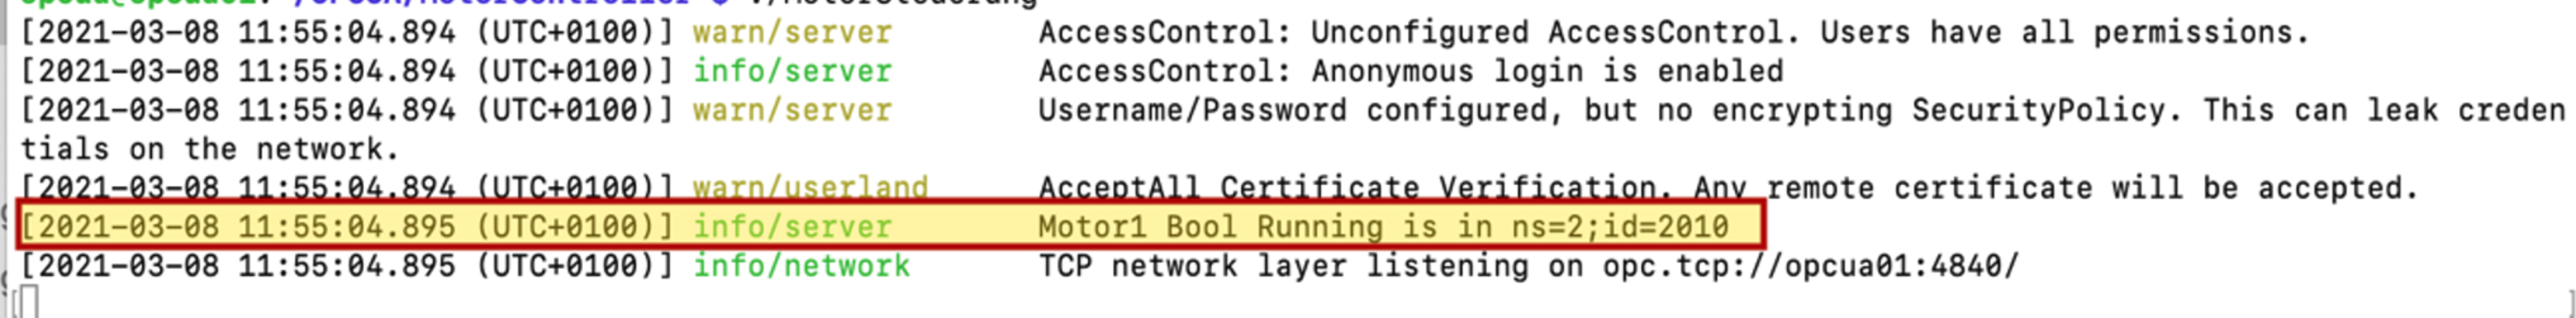
\includegraphics[width=1\linewidth]{abb/ServerRunMotor}
	\caption{Log Ausgabe der abgefragten Node-ID}
	\label{fig:serverrunmotor}
\end{figure}

Wenn ja, können wir noch prüfen, ob im UA Expert Client alles erwartungsgemäß angezeigt wird
\clearpage
\section{Methoden und Variable mit Logic verbinden}
Nachdem nun ein funktionierender Server-Code vorliegt, wird mit dem Anlegen der Lo-gic für Variable und Methoden begonnen.

\subsection{Ändern der Server-Laufzeit-Routine}
Derzeit wird der Server mit
\begin{lstlisting}[language=Bash]
UA_Server_run(server, &running);
\end{lstlisting}
gestartet. Dieser Aufruf wird solange durchgeführt, bis die Variable running auf false gesetzt wird. Wenn wir allerdings nun während der Ausführung des Servers noch andere Aktionen ausführen wollen, z.B. das lesen eines Sensors und schreiben einer OPC UA Variable während des Vorgangs müssen wir die Server Routine ein wenig verändern (im Kapitel \autoref{sec:callbacks-fur-variablen} kommen wir allerdings zu noch einer anderen Möglichkeit).
Dies tun wir indem diese Zeile aus der main.c entfernen und den Code mit Folgendem erweitern.
\begin{lstlisting}[language=Bash]
retval = UA_Server_run_startup(server);
//https://open62541.org/doc/current/server.html#server-lifecycle
if(retval != UA_STATUSCODE_GOOD) {
	UA_Server_delete(server);
	return retval;
}
while(running == true)
{
	//Server Routine
	//https://open62541.org/doc/current/server.html#server-lifecycle
	UA_Server_run_iterate(server, true);
}

return retval == UA_STATUSCODE_GOOD ? EXIT_SUCCESS : EXIT_FAILURE;
\end{lstlisting}
Hier sieht man, dass wir dem Server zunächst die Startup-Routine durchlaufen lassen, prüfen, ob dies erfolgreich war und dann eine while-Schleife starten, in der wir bei jedem Durchlauf einmal die Server-Routine durchlaufen.

\subsection{Variable}
Um nun z.B. in der while-Schleife jede Sekunde den speed um 1 zu erhöhen und alle 5 Sekunden den Zustand des bool running zu ändern, ergänzen wir den Code folgendermaßen.
Wichtig: Hierfür muss noch \#include <time.h> hinzugefügt werden.
\begin{lstlisting}[language=Bash]
int timestampM1Running = time(0) + 2;
int timestampM1Speed = time(0) + 1;
//https://open62541.org/doc/current/types.html
UA_Boolean m1running = false;
UA_Int16 m1speed = 0;
while(running == true)
{
	//Server Routine https://open62541.org/doc/current/server.html#server-lifecycle
	UA_Server_run_iterate(server, true);
	
	//Multi Use Variables for Update
	int time_now = time(0);
	UA_Variant value;
	
	//Update Variable Running every 2s
	if(time_now > timestampM1Running)
	{
		timestampM1Running = time_now + 2;
		m1running = m1running ? false : true;
		//https://open62541.org/doc/current/plugin_log.html
		UA_LOG_INFO(UA_Log_Stdout, UA_LOGCATEGORY_USERLAND,
		"New Motor 1 Running Bool: %s",m1running ? "True" : "False");
		//https://open62541.org/doc/current/types.html#generated-data-type-definitions
		//https://open62541.org/doc/current/types.html#variant
		UA_Variant_setScalar(&value, &m1running,&UA_TYPES[UA_TYPES_BOOLEAN]);
		
		//https://open62541.org/doc/current/server.html#reading-and-writing-node-attributes	
		UA_Server_writeValue(server, UA_NODEID_NUMERIC(nsIdx, 2010), val-ue);
	}
	
	//Update Variable Speed every 1s
	if(time_now > timestampM1Speed)
	{
		timestampM1Speed = time_now + 1;
		m1speed++;
		UA_LOG_INFO(UA_Log_Stdout, UA_LOGCATEGORY_USERLAND,
		"New M1 Speed int: %d", m1speed);
		UA_Variant_setScalar(&value, &m1speed,  &UA_TYPES[UA_TYPES_INT16]);
		UA_Server_writeValue(server, UA_NODEID_NUMERIC(nsIdx, 2011), val-ue);
	}
}

return retval == UA_STATUSCODE_GOOD ? EXIT_SUCCESS : EXIT_FAILURE;
\end{lstlisting}
Im Code sind auch die Verweise verzweigt, wo man dies in der Dokumentation findet. Wichtig ist zu wissen, dass zum Schreiben einer Variable das Erstellen einer Variante nötig ist. In dieser werden später der gewünschte Wert und die Information des Datentyps temporär abgespeichert und zwar mit der Function UA\_Variant\_setScalar.
Diese Variante kann man dann mit der Funktion UA\_Server\_writeValue schreiben,
die einen Pointer auf dem Server benötigt, die nötige Node-ID und die soeben erstellte Variante.

\subsection{Methoden}
Methoden benötigen eine Callback-Funktion. Wir erstellen diese vor der Main-Methode
exemplarisch für die Methode Control.
\begin{lstlisting}[language=Bash]
static UA_StatusCode
ControlMethodCallback(UA_Server *server,
const UA_NodeId *sessionId, void *sessionHandle,
const UA_NodeId *methodId, void *methodContext,
const UA_NodeId *objectId, void *objectContext,
size_t inputSize, const UA_Variant *input,
size_t outputSize, UA_Variant *output) {
	//Handle Input
	UA_Int16 speed_in = *(UA_Int16*)input[0].data;
	UA_Int16 distance_in = *(UA_Int16*)input[1].data;
	UA_Boolean direction_in = *(UA_Boolean*)input[2].data;
	
	//Handle Direction and set for test the return Value to direction value
	UA_Boolean ret_val = direction_in;
	UA_Variant value;
	UA_Variant_setScalar(&value, &ret_val, &UA_TYPES[UA_TYPES_BOOLEAN]);
	UA_Server_writeValue(server, UA_NODEID_NUMERIC(nsIdx, 2012), value);
	
	//Return the Value to Methode Output
	UA_Variant_setScalarCopy(output, &ret_val, &UA_TYPES[UA_TYPES_BOOLEAN]);
	
	//End Methode
	UA_LOG_INFO(UA_Log_Stdout, UA_LOGCATEGORY_SERVER, "Control was called");
	return UA_STATUSCODE_GOOD;
}
\end{lstlisting}
Um zu sehen, in welcher Reihenfolge die Input-Parameter abzurufen sind, kann man ei-nen Blick in sein Modell werfen. Wie in Abbildung \autoref{fig:inputargumente} zu sehen, kann man im Attributes Editor die Argumente unter Values identifizieren.
\begin{figure}[H]
	\centering
	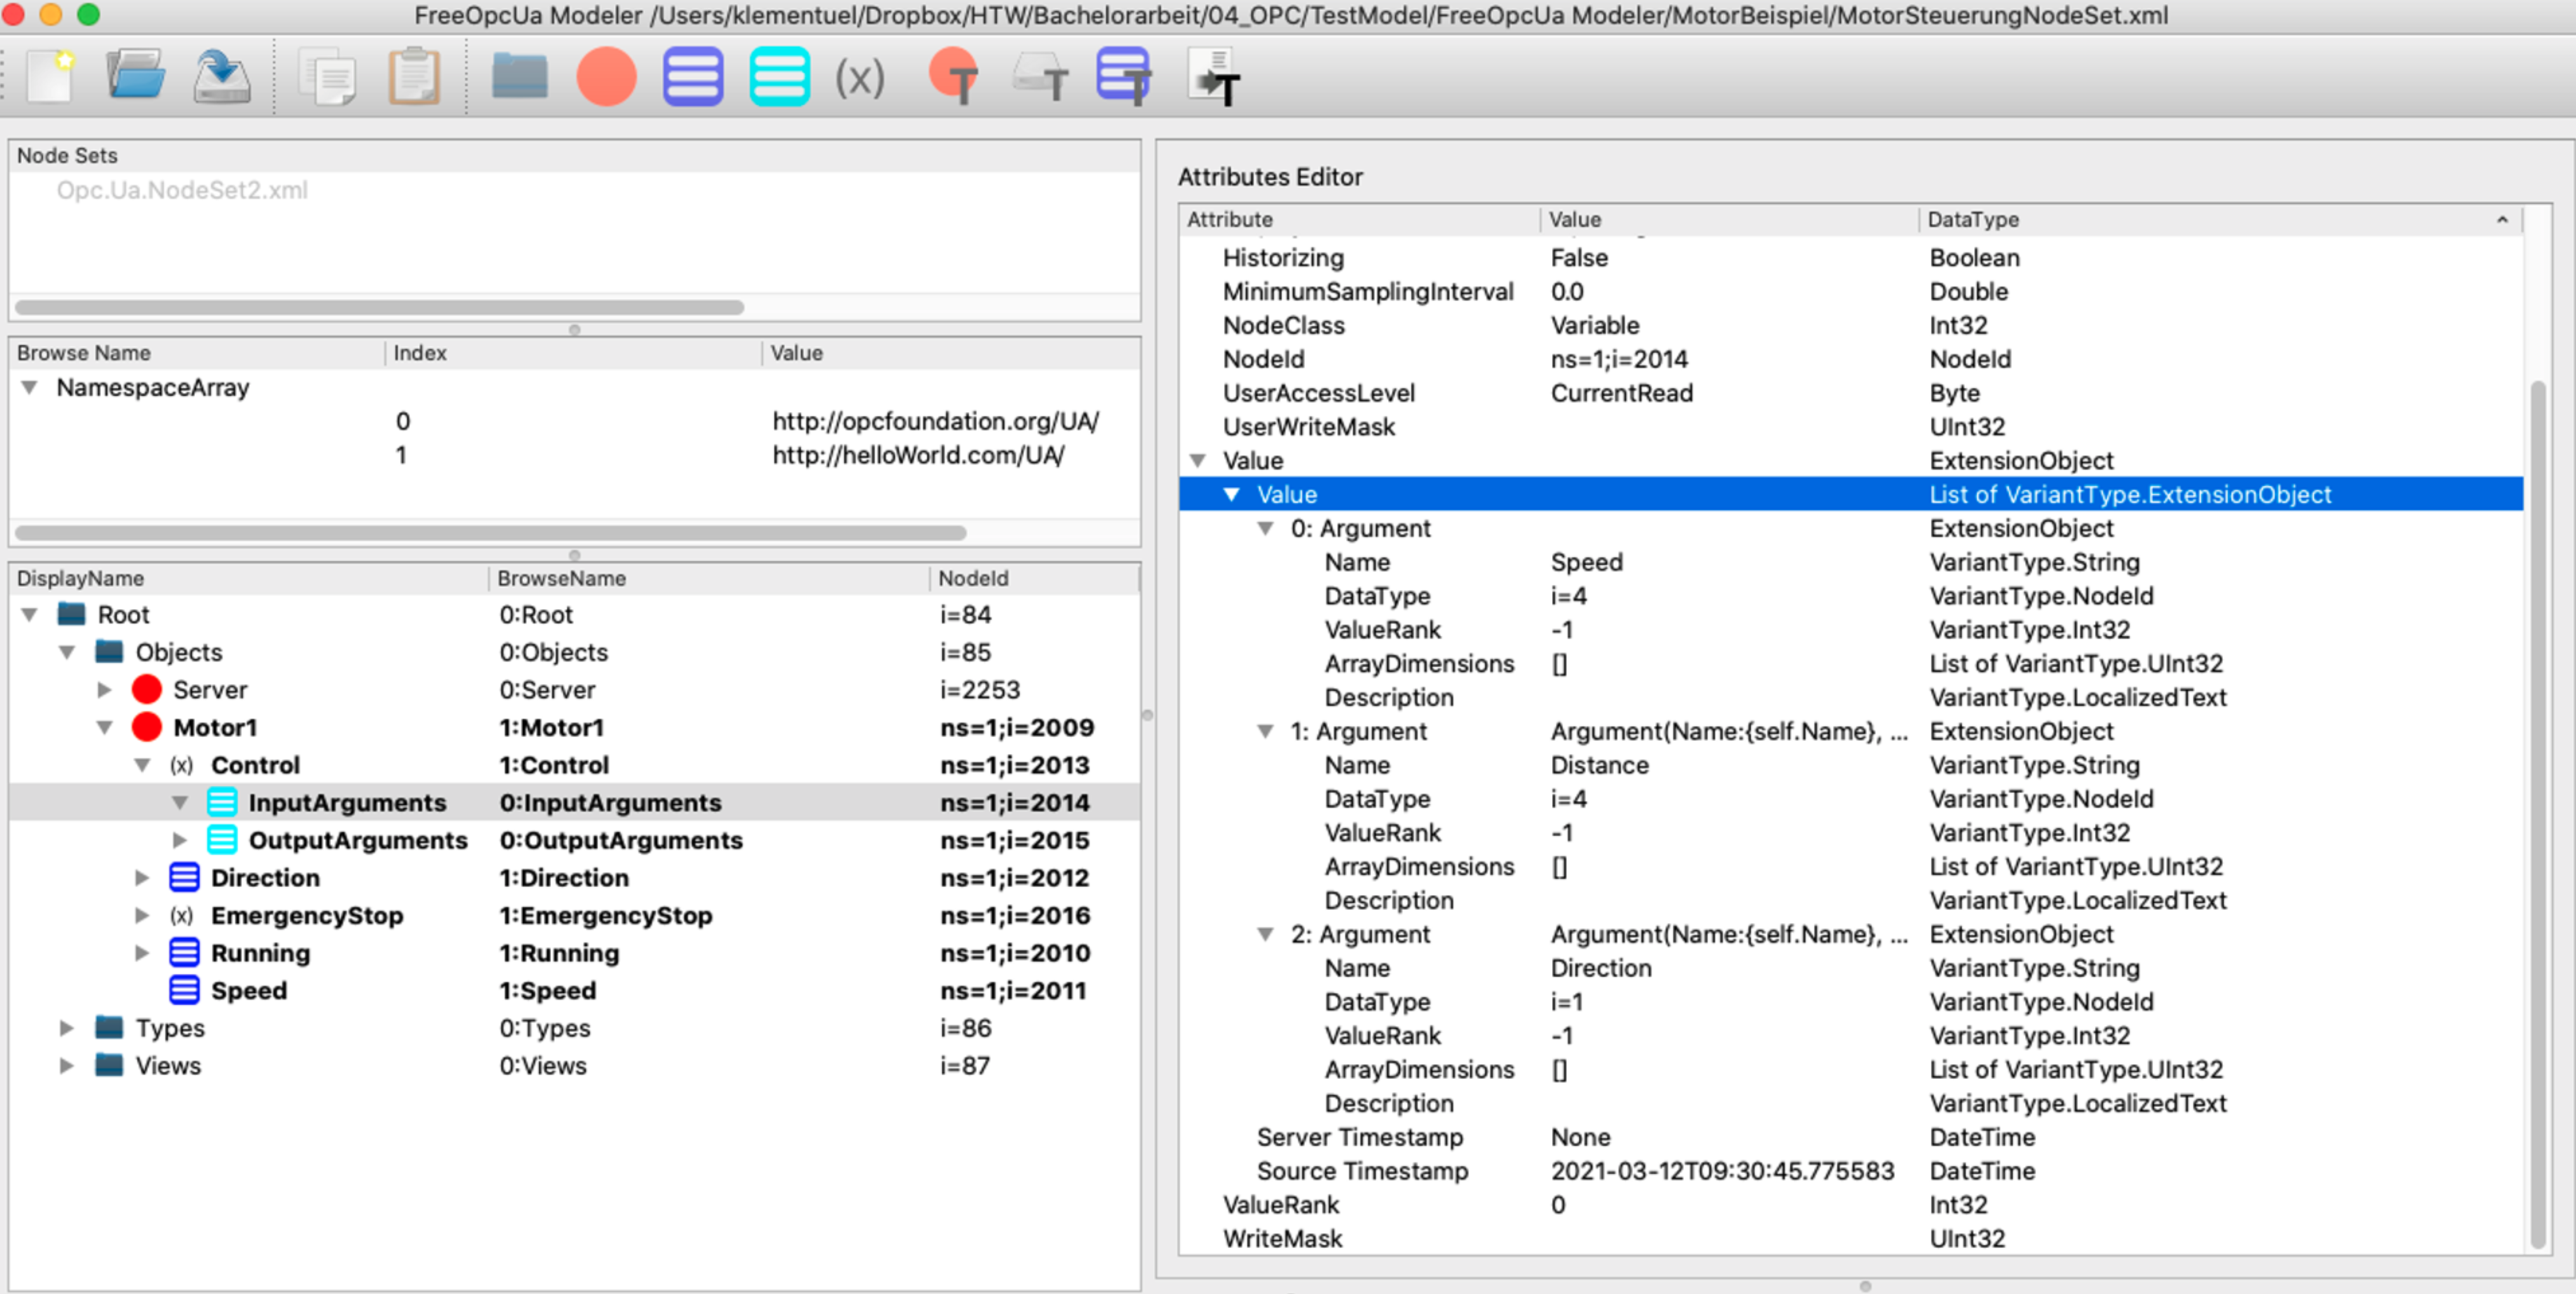
\includegraphics[width=1\linewidth]{abb/InputArgumente}
	\caption{Anzeige Reihenfolge Input-Argumente}
	\label{fig:inputargumente}
\end{figure}



Damit kann man dann lokale Variable schreiben und seine Methoden Logic durchführen. Wir schreiben in diesem Fall einfach nur den Input Direction direkt in die Server Variable Direction und ändern damit auch je nach dem die output-Variable mit UA\_Variant\_setScalarCopy.

Im nächsten Schritt müssen wir der Methode noch sagen, dass sie diesen ein Callback aufrufen soll. Dies geschieht mit folgender Erweiterung in der Main-Methode.

\begin{lstlisting}[language=Bash]
//Set Callback for M1 Control https://open62541.org/doc/1.2/server.html#method-callbacks
UA_Server_setMethodNode_callback(server,
UA_NODEID_NUMERIC(nsIdx, 2013),
&ControlMethodCallback);
\end{lstlisting}
Diesen Code-Teil kann man nach dem Server-Startup implementieren.

\subsection{Modifizierte main.c}

Hier findet man noch die gesamten Änderungen der main.c zusammengefasst.
\begin{lstlisting}[language=Bash]
#include <open62541/plugin/log_stdout.h>
#include <open62541/server.h>
#include <open62541/server_config_default.h>
#include <signal.h>
#include <stdlib.h>
#include "MotorSteuerung.h"

#include <time.h>

UA_Boolean running = true;
UA_UInt16 nsIdx; //Namespace  "http://helloWorld.com/UA/"

static UA_StatusCode
ControlMethodCallback(UA_Server *server,
const UA_NodeId *sessionId, void *sessionHandle,
const UA_NodeId *methodId, void *methodContext,
const UA_NodeId *objectId, void *objectContext,
size_t inputSize, const UA_Variant *input,
size_t outputSize, UA_Variant *output) {
	//Handle Input
	UA_Int16 speed_in = *(UA_Int16*)input[0].data;
	UA_Int16 distance_in = *(UA_Int16*)input[1].data;
	UA_Boolean direction_in = *(UA_Boolean*)input[2].data;
	
	//Handle Direction and set for test the return Value to direction value
	UA_Boolean ret_val = direction_in;
	UA_Variant value;
	UA_Variant_setScalar(&value, &ret_val, &UA_TYPES[UA_TYPES_BOOLEAN]);
	UA_Server_writeValue(server, UA_NODEID_NUMERIC(nsIdx, 2012), value);
	
	//Return the Value to Methode Output
	UA_Variant_setScalarCopy(output, &ret_val, &UA_TYPES[UA_TYPES_BOOLEAN]);
	
	//End Methode
	UA_LOG_INFO(UA_Log_Stdout, UA_LOGCATEGORY_SERVER, "Control was called");
	return UA_STATUSCODE_GOOD;
}

static void stopHandler(int sign) {
	UA_LOG_INFO(UA_Log_Stdout, UA_LOGCATEGORY_SERVER, "received ctrl-c");
	running = false;
}

int main(int argc, char** argv) {
	signal(SIGINT, stopHandler);
	signal(SIGTERM, stopHandler);
	
	UA_Server *server = UA_Server_new();
	UA_ServerConfig_setDefault(UA_Server_getConfig(server));
	UA_StatusCode retval;
	/* create nodes from nodeset */
	if(MotorSteuerung(server) != UA_STATUSCODE_GOOD) {
		UA_LOG_ERROR(UA_Log_Stdout, UA_LOGCATEGORY_SERVER, "Could not add the Motor-Steuerung nodeset. "
		"Check previous output for any error.");
		retval = UA_STATUSCODE_BADUNEXPECTEDERROR;
	} else {
		// Do some additional stuff with the nodes
		// this will just get the namespace index, since it is already added to the server
		nsIdx = UA_Server_addNamespace(server, "http://helloWorld.com/UA/");
		// UA_MOTOR1_RUNNING_BOOL = 2010
		UA_NodeId testInstanceId = UA_NODEID_NUMERIC(nsIdx, 2010);
		UA_LOG_INFO(UA_Log_Stdout, UA_LOGCATEGORY_SERVER, "Motor1 Bool Running is in ns=%d;id=%d",
		testInstanceId.namespaceIndex, testIn-stanceId.identifier.numeric);
		
	}
	//
	retval = UA_Server_run_startup(server);
	//Set Callback for M1 Control https://open62541.org/doc/1.2/server.html#method-callbacks
	UA_Server_setMethodNode_callback(server,
	UA_NODEID_NUMERIC(nsIdx, 2013),
	&ControlMethodCallback);
	
	//https://open62541.org/doc/current/server.html#server-lifecycle
	if(retval != UA_STATUSCODE_GOOD) {
		UA_Server_delete(server);
		return retval;
	}
	
	int timestampM1Running = time(0) + 2;
	int timestampM1Speed = time(0) + 1;
	//https://open62541.org/doc/current/types.html
	UA_Boolean m1running = false;
	UA_Int16 m1speed = 0;
	while(running == true)
	{
		//Server Routine https://open62541.org/doc/current/server.html#server-lifecycle
		UA_Server_run_iterate(server, true);
		
		//Multi Use Variables for Update
		int time_now = time(0);
		UA_Variant value;
		
		//Update Variable Running every 2s
		if(time_now > timestampM1Running) {
			timestampM1Running = time_now + 2;
			m1running = m1running ? false : true;
			//https://open62541.org/doc/current/plugin_log.html
			UA_LOG_INFO(UA_Log_Stdout, UA_LOGCATEGORY_USERLAND, "New Motor 1 Running Bool: %s",
			m1running ? "True" : "False");
			//https://open62541.org/doc/current/types.html#generated-data-type-definitions
			//https://open62541.org/doc/current/types.html#variant
			UA_Variant_setScalar(&value, &m1running,  &UA_TYPES[UA_TYPES_BOOLEAN]);
			
			//https://open62541.org/doc/current/server.html#reading-and-writing-node-attributes
			UA_Server_writeValue(server, UA_NODEID_NUMERIC(nsIdx, 2010), value);
		}
		
		//Update Variable Speed every 1s
		if(time_now > timestampM1Speed) {
			timestampM1Speed = time_now + 1;
			m1speed++;
			UA_LOG_INFO(UA_Log_Stdout, UA_LOGCATEGORY_USERLAND, "New M1 Speed int: %d",
			m1speed);
			UA_Variant_setScalar(&value, &m1speed,  &UA_TYPES[UA_TYPES_INT16]);
			UA_Server_writeValue(server, UA_NODEID_NUMERIC(nsIdx, 2011), value);
		}
	}
	
	return retval == UA_STATUSCODE_GOOD ? EXIT_SUCCESS : EXIT_FAILURE;
}
\end{lstlisting}

\subsection{Kompilieren und testen}
Nun kann der Code wie im Kapitel 6 kompiliert und getestet werden.

In UA Expert kann man sich die Variablen in das Data Access View-Fenster ziehen und beobachten, wie sich der Wert ändert. 
Die Methode kann mit einem rechten Mausklick aufgerufen werden, danach kann man die Input-Parameter setzen und mit Call den Abruf erledigen. Hier sind nun die Änderungen der Direction und Success zu beobachten. In \autoref{fig:abrufmethode} sieht man einen erfolgreichen Methoden-Aufruf.

\begin{figure}[H]
	\centering
	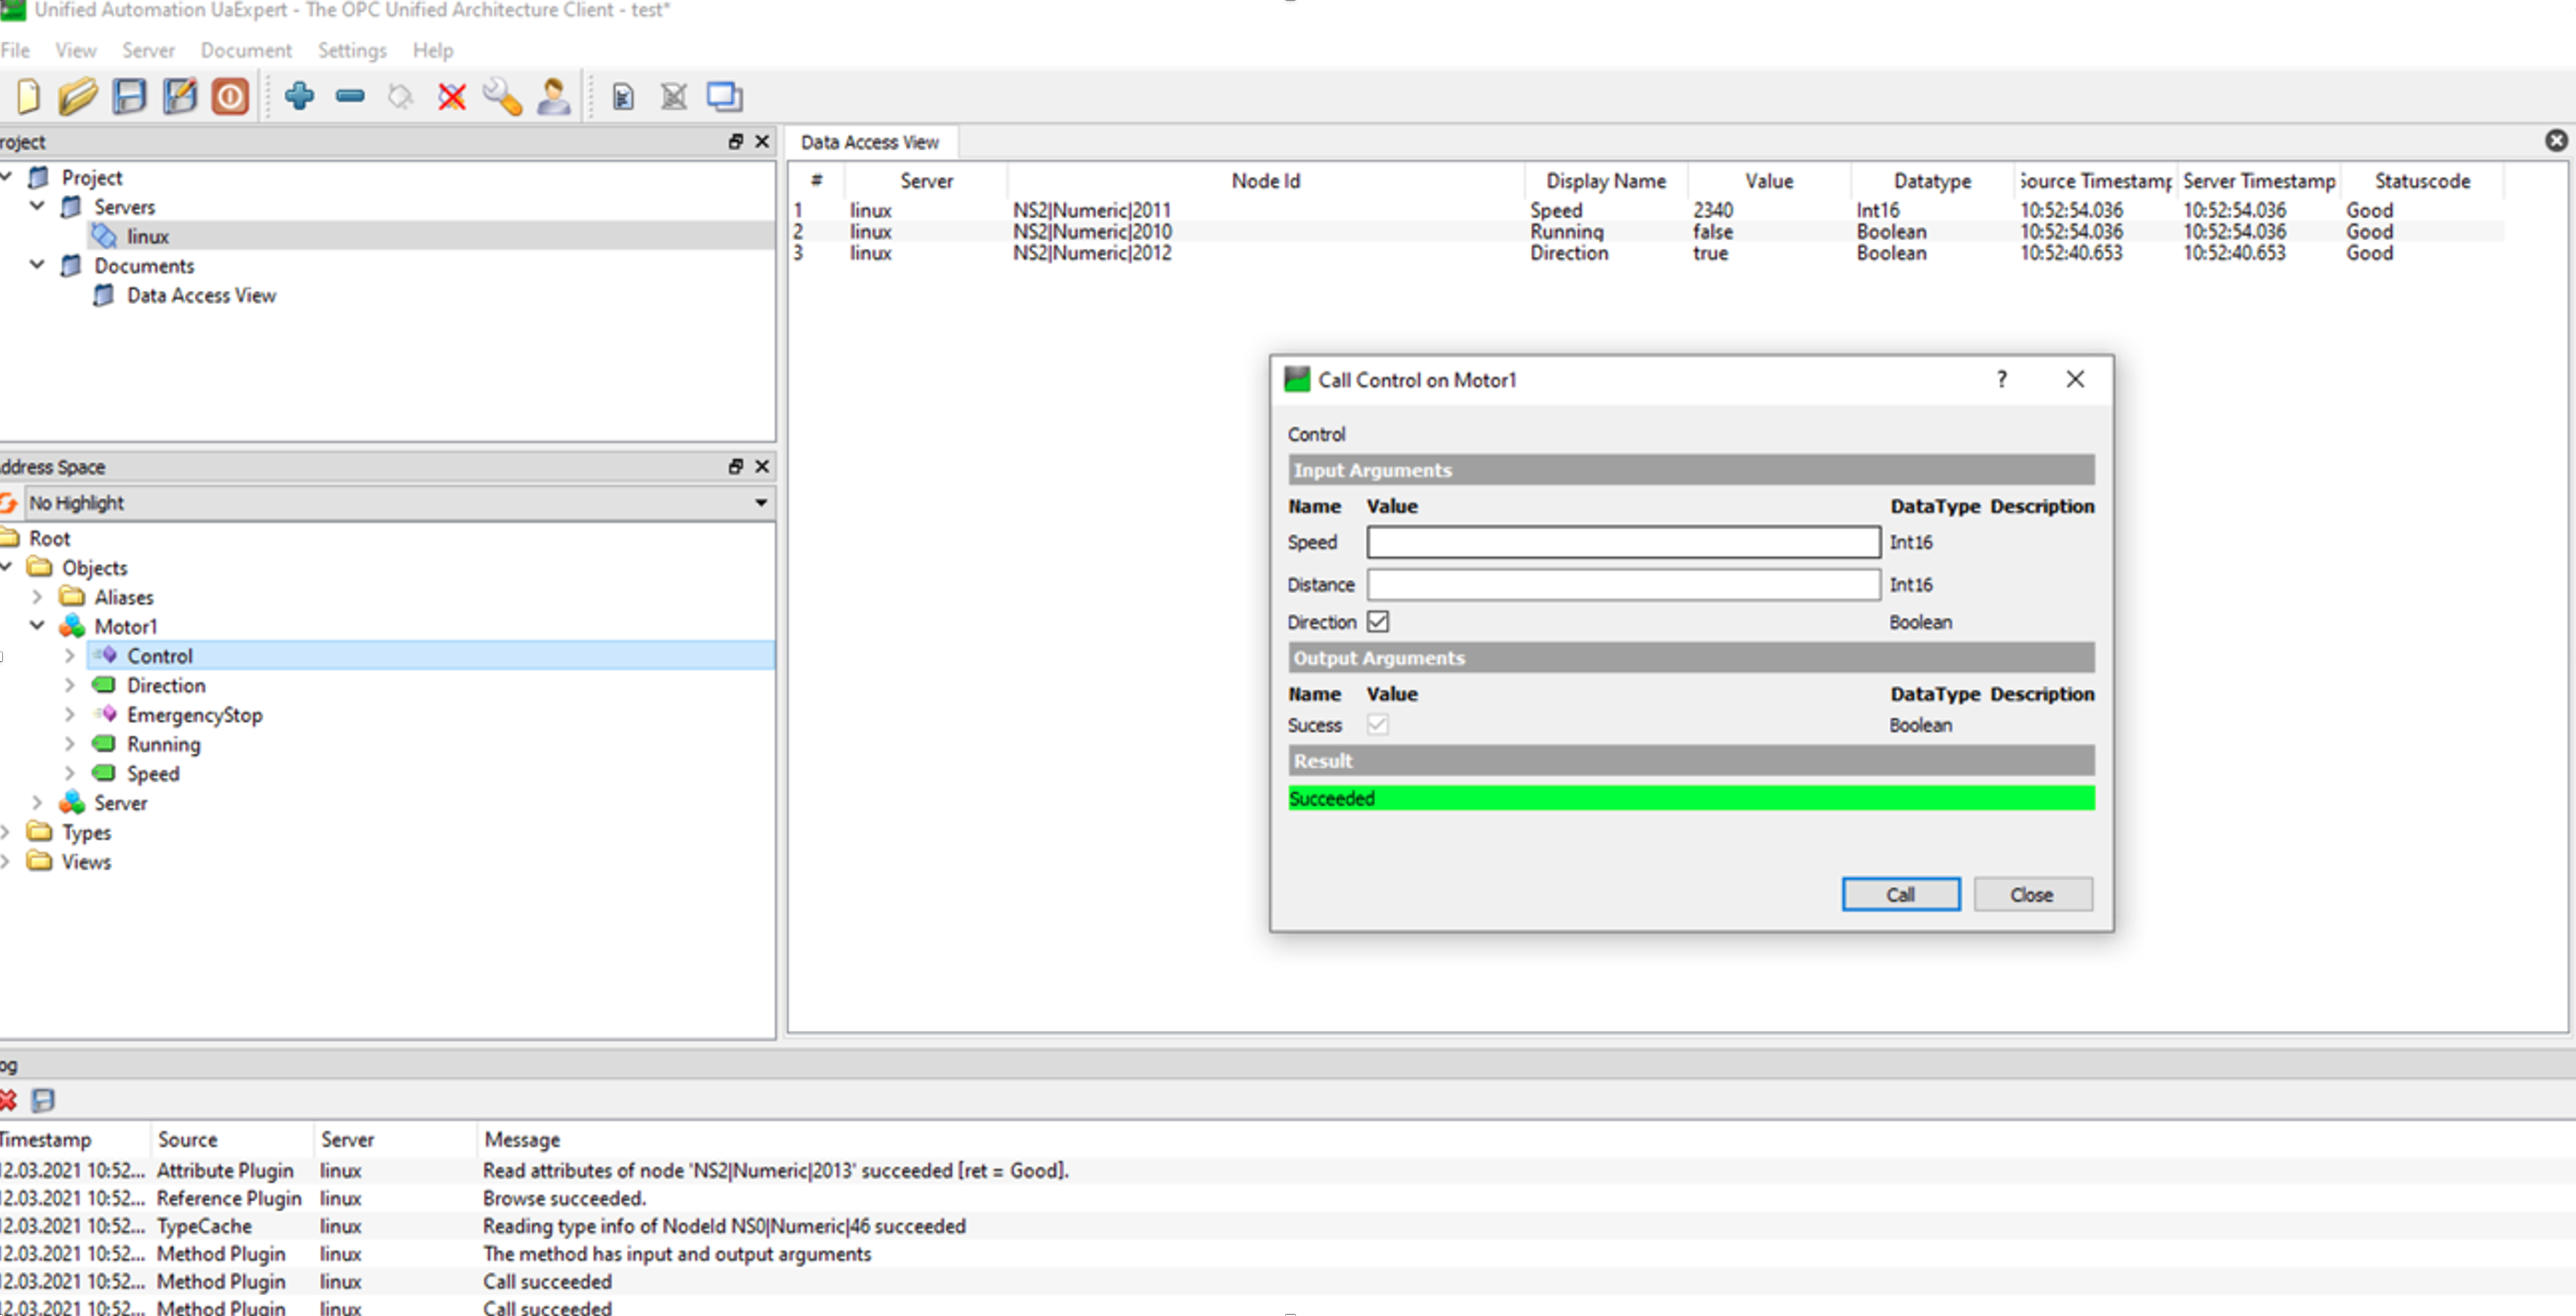
\includegraphics[width=1\linewidth]{abb/AbrufMethode}
	\caption{Abruf von Methoden}
	\label{fig:abrufmethode}
\end{figure}
\clearpage
\section{Fortgeschritten Erweiterungen}
In diesem Kapitel wollen wir nur auf weitere Möglichkeiten eingehen, wie man mit Variablen vor oder nach dem Lesen bzw. Schreiben Aktionen auslöst, wie man Methoden, die durch lange Operationen den Server blockieren würden, asynchron bekommt oder die Möglichkeit die Schematische Struktur seines Servers zu durchsuchen ohne die NodeID´s einzelner Objekte zu kennen. Hierzu dient uns ein Beispiel aus der Bachelor Arbeit des Umsetzungsteils des PaintingStationBelt.
Dieses Beispiel ist vom Aufbau schon ein wenig komplexer in seiner Strukturiert um allerdings auch die Übersicht zu vereinfachen wie in \autoref{fig:open62541server} zu sehen.
\begin{figure}[H]
	\centering
	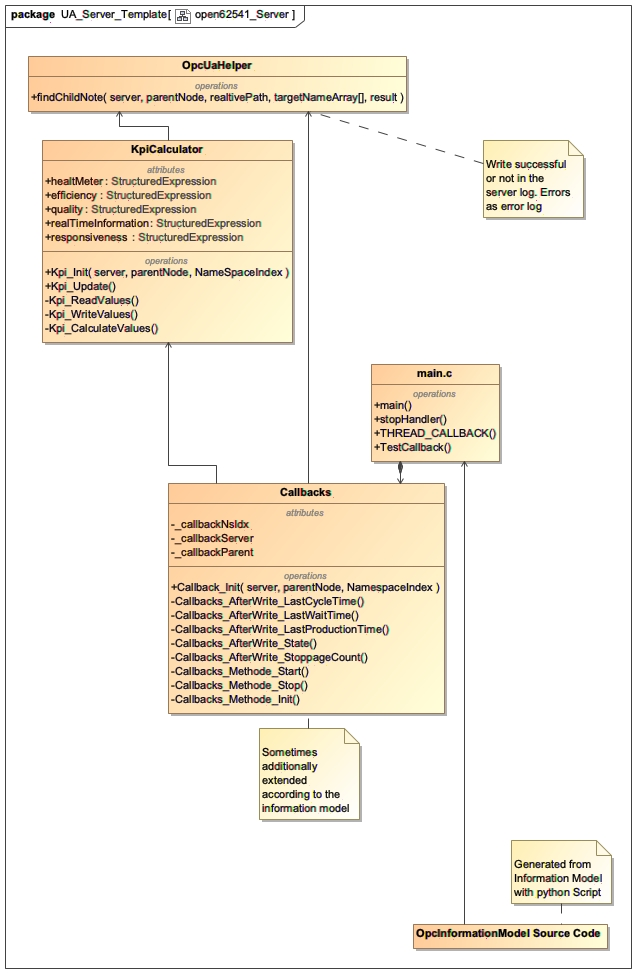
\includegraphics[width=1\linewidth]{abb/open62541_Server}
	\caption{Klassendiagram Painting Staion Belt}
	\label{fig:open62541server}
\end{figure}
In \autoref{fig:konopc-ua-information-model-belt} sieht man dazu auch eine Übersicht des OPC UA Informationsmodels, allerdings nicht in der empfohlenen Schematischen Modellierung der OPC UA Fundation, da dies in der Bachelor Arbeit mit SysML modelliert wurde.

\begin{figure}[H]
	\centering
	\includegraphics[width=1\linewidth]{"abb/konOPC UA Information Model Belt"}
	\caption{MBSE Informationsmodel}
	\label{fig:konopc-ua-information-model-belt}
\end{figure}

\subsection{Callbacks für Variablen}\label{sec:callbacks-fur-variablen}
Wie schon bei den Methoden ist es möglich Callbacks für Variablen zu setzen. Entweder das diese eine Aktion auslösen, bevor sie gelsen werden, oder nachdem sie beschrieben wurden.
Im Beispiel wollen wir nun das nach dem schreiben der Variable, der Status eine Server Log Nachricht ausgibt. Dazu schreiben wir als erstes eine passende Funktion 
\begin{lstlisting}[language=C]
	void 
	Callbacks_AfterWrite_State(UA_Server *server,
	const UA_NodeId *sessionId, void *sessionContext,
	const UA_NodeId *nodeId, void *nodeContext,
	const UA_NumericRange *range, const UA_DataValue *data)
	{
		UA_LOG_INFO(UA_Log_Stdout, UA_LOGCATEGORY_SERVER, "State has Changed");
	}        
\end{lstlisting}
nun müssen wir dem Server noch das Callback zuordnen
\begin{lstlisting}[language=C]
	/*Create and set the appropriate methods in the Callback variable. Important if you don't assign a function you have to set NULL, otherwise unexpected pointer errors can occur.*/
	UA_ValueCallback callback;
	callback.onRead = NULL;
	callback.onWrite = Callbacks_AfterWrite_State;
	//Set the callback variable to the NodeID
	UA_Server_setVariableNode_valueCallback(server, 
	variable_State,
	callback);
\end{lstlisting}

Damit ist das ganze schon erledigt und einsatzbereit.
\subsection{Methoden mit Multithreading}
Man kann sich sicher Vorstellen, dass es auch Callbacks gibt die den Server blockieren können, da diese eine gewisse Zeit benötigen um zu einem Ergebnis zu kommen.
Wie z.B. in meiner Bachelor Arbeit. Hier wurden Python Scripts von Methoden aufgerufen, die z.B. im Fall von dem PaintingStationBelt gut 10s für einen Aufruf benötigen. In dieser Zeit kann ein Client keine Variablen schreiben oder lesen, das natürlich dann zu Fehlern führen würde. Zum Glück gibt es bei open62541 SDK die Option Multithreading zu aktivieren. Dazu müsst ihr das SDK mit der entsprechenden Option im ccmake unter UA\_Multithreading = 100 setzen und neu bauen.  Der Rest bleibt gleich wie in \autoref{sec:open62541} beschrieben

Beginnend im main.c File musste man dann folgendes erweitern in der \#Include Sektion:
\begin{lstlisting}[language=C]
	#ifndef WIN32
	#include <pthread.h>
	#define THREAD_HANDLE pthread_t
	#define THREAD_CREATE(handle, callback) pthread_create(&handle, NULL, callback, NULL)
	#define THREAD_JOIN(handle) pthread_join(handle, NULL)
	#define THREAD_CALLBACK(name) static void * name(void *_)
	#else
	#include <windows.h>
	#define THREAD_HANDLE HANDLE
	#define THREAD_CREATE(handle, callback) { handle = CreateThread( NULL, 0, callback, NULL, 0, NULL); }
	#define THREAD_JOIN(handle) WaitForSingleObject(handle, INFINITE)
	#define THREAD_CALLBACK(name) static DWORD WINAPI name( LPVOID lpParam )
	#endif
\end{lstlisting}
Und mit zwei Funktionen vor der main Funktion erweitern.

\begin{lstlisting}[language=C]
THREAD_CALLBACK(ThreadWorker) {
	while(running) {
		UA_LOG_INFO(UA_Log_Stdout, UA_LOGCATEGORY_SERVER,
		"Try to dequeue an async operation");
		const UA_AsyncOperationRequest* request = NULL;
		void *context = NULL;
		UA_AsyncOperationType type;
		if(UA_Server_getAsyncOperationNonBlocking(server, &type, &request, &context, NULL) == true) {
			UA_LOG_INFO(UA_Log_Stdout, UA_LOGCATEGORY_SERVER, "AsyncMethod_Testing: Got entry: OKAY");
			UA_CallMethodResult response = UA_Server_call(server, &request->callMethodRequest);
			UA_Server_setAsyncOperationResult(server, (UA_AsyncOperationResponse*)&response,
			context);
			UA_LOG_INFO(UA_Log_Stdout, UA_LOGCATEGORY_SERVER, "AsyncMethod_Testing: Call done: OKAY");
			UA_CallMethodResult_clear(&response);
		} else {
			/* not a good style, but done for simplicity :-) */
			sleep(5);
		}
	}
	return 0;
}

/* This callback will be called when a new entry is added to the Callrequest queue */
static void
TestCallback(UA_Server *server) {
	UA_LOG_INFO(UA_Log_Stdout, UA_LOGCATEGORY_SERVER,
	"Dispatched an async method");
}
\end{lstlisting}
Das war schon der schwierigste Teil, im nächsten Schritt fügen wir in der Callback.c Datei noch den Eintrag hinzu, dass dieses Callback Asynchron ausgeführt werden muss.

\begin{lstlisting}[language=C]
UA_Server_setMethodNode_callback(server,
methode_Start,
&Callbacks_Methode_Start);
UA_Server_setMethodNodeAsync(server, methode_Start, UA_TRUE);
\end{lstlisting}

Nun kann man die Methoden Asynchron aufrufen.

\subsection{Browse}
Ein wichtiger Grund, warum man überhaupt ein Informationsmodel braucht ist die Möglichkeit Schematisch Objekte abzufragen. also das ich wie in einer Ordner Struktur Stück für Stück nach dem richtigen Eintrag suchen kann. Dazu hatte ich ihn der Bachelor Arbeit eine kleine Helfer Funktion geschrieben, mit der man dann auch Fehler einer Anfrage Filtern kann bzw. auch die erfolgreichen Abfragen im Server Log sieht.

Als erstes wird ein Array, das die tiefer der Abfrage entspricht, angelegt als Typ UA\_Qualified Name. In diesem Fall suchen wir in unserem Hauptobjekt den Ordner Control und danach die Methode Test

\begin{lstlisting}[language=C]
UA_QualifiedName targetNameArr[2] = {UA_QUALIFIEDNAME(*_callbackNsIdx, "Control"), 
UA_QUALIFIEDNAME(*_callbackNsIdx, "Test"), 
\end{lstlisting}
Danach müssen wir definieren, von wo wir anfangen zu suchen, also das Parent Objekt in dem Fall PaintingStationBelt, hier wissen wir die NodeID, natürlich ist auch eine Abfrage aus dem Root Ordner möglich, also wenn selbst die NodeID des Hauptobjekt unbekannt ist.
\begin{lstlisting}[language=C]
UA_NodeId parent = UA_NODEID_NUMERIC(nsIdx, 3001);
\end{lstlisting}
Dann benötigen wir auch eine NodeID, wo wir die Abfrage speichern wollen in diesem Fall 
\begin{lstlisting}[language=C]
UA_NodeId methode_Test;
\end{lstlisting}
und können nun die Abfrage vollziehen mit der Helfer Funktion
\begin{lstlisting}[language=C]
findChildNode(server, *parent, 2, targetNameArr, &methode_Test);
\end{lstlisting}
Nach der Abfrage gibt sie eine Rückmeldung als Server Log und beschreibt die NodeID Variable mit der man nun weiter arbeiten kann.

Nur was macht diese Helfer Funktion?
Dies schauen wir uns nun an.
\begin{lstlisting}[language=C]
int findChildNode(UA_Server *server, 
UA_NodeId parentNode, 
const int relativePathCnt, 
UA_QualifiedName targetNameArr[], 
UA_NodeId *result) 
{
	int ret = 0;
	
	UA_BrowsePathResult bpr = UA_Server_browseSimplifiedBrowsePath(server, 
	parentNode, relativePathCnt, targetNameArr);
	
	if (bpr.statusCode != UA_STATUSCODE_GOOD || bpr.targetsSize < 1)
	{
		char msg[200];
		strcpy(msg, "Find Child Error from: ");
		for(int tragets = 0; tragets < relativePathCnt; tragets++)
		{
			strcat(msg, "/");
			strcat(msg, (char*)targetNameArr[tragets].name.data);
		}
		strcat(msg, " With status Code: "); 
		strcat(msg, UA_StatusCode_name(bpr.statusCode));
		UA_LOG_WARNING(UA_Log_Stdout, UA_LOGCATEGORY_SERVER, msg);
		ret = -1;
	}
	else
	{
		UA_NodeId_copy(&bpr.targets[0].targetId.nodeId, result);
		char msg[200];
		strcpy(msg, "Child found:  ");
		for(int tragets = 0; tragets < relativePathCnt; tragets++)
		{
			strcat(msg, "/");
			strcat(msg, (char*)targetNameArr[tragets].name.data);
		}
		UA_LOG_INFO(UA_Log_Stdout, UA_LOGCATEGORY_SERVER, msg);
	}
	
	
	UA_BrowsePathResult_clear(&bpr);
	
	return ret;
}
\end{lstlisting}
Diese kann nun nach Belieben ergänzt werden um z.B. den Exception handling des Servers gerecht zu werden.
\clearpage
\section{Custom Cmake File}
Der bis jetzt benutzte gcc Befehl ist natürlich nur eine Möglichkeit sein Server zu kompilieren, allerdings da der Server mit der Zeit komplexer wird, mehr Dateien einzubinden sind, kann es schon mühselig werden diesen Befehl jedes Mal zu schrieben oder zu suchen und zu kopieren.
Deshalb werden wir uns nun mit CMake auseinander setzen.

In unserem einfachen Beispiel des Motor Controller erstellen wir uns in dessen Pfad, deshalb eine Datei mit
\begin{lstlisting}[language=Bash]
nano CMakeLists.txt
\end{lstlisting}
und in dieser schreiben wir folgendes
\begin{lstlisting}[language=make]
make_minimum_required(VERSION 3.10)

# set the project name
project(MotorSteuerung)

set(CMAKE_PREFIX_PATH "/home/parallels/install")
message("Cmake Prefix Path is \"${CMAKE_PREFIX_PATH}\"")
# open62541 must be installed.
# If in custom path, then use -DCMAKE_PREFIX_PATH=/home/user/install
# Set with Required Components the Namespace like FullNamespace or ReducedNamespace
find_package(open62541 1.1 REQUIRED COMPONENTS FullNamespace)

#The following folder will be included
include_directories(${CMAKE_PREFIX_PATH}/include)
link_directories(${CMAKE_PREFIX_PATH}/lib)

# add the executable
add_executable(MotorSteuerung main.c MotorSteuerung.c)

#The following libraries will be linked
target_link_libraries(MotorSteuerung open62541 mbedtls mbedx509 mbedcrypto)

#Limit Parallel Linking Jobs with -DMY_LIMIT_FLAG=ON
option(MY_LIMIT_FLAG "If Build fail you can set this ON to Limit parralel Linking Jobs to One" OFF) #OFF by default
if(MY_LIMIT_FLAG)
set(MY_LIMIT_FLAG "-flto=1")
message("Set Parallel Linking Jobs to One")
endif(MY_LIMIT_FLAG)
unset(MY_LIMIT_FLAG CACHE) # <---- this is the important!!

#Set the the C Standart
set_property(TARGET MotorSteuerung PROPERTY C_STANDARD 99)
\end{lstlisting}
dies speichern wir mit dem Befehl Control x 
danach erstellen wir den Ordner build und wechseln in diesen mit
\begin{lstlisting}[language=Bash]
mkdir build && cd build
\end{lstlisting}
nun können wir die benötigten Build Artefakte für Cmake erstellen mit der Eingabe
\begin{lstlisting}[language=Bash]
cmake .. -DCMAKE_PREFIX_PATH=/home/{user}/install -DMY_LIMIT_FLAG=ON
\end{lstlisting}
und nach dem erfolgreichen Abschluss kann das Projekt gebaut werden mit
\begin{lstlisting}[language=Bash]
make -j
\end{lstlisting}
Solange sich nun am CMakeLists.txt File nichts ändert können immer wieder neue Server Versionen bei Änderungen der Source Files mit make -j erstellt werden.

Man kann noch andere Bibliotheken und Klassen einbinden wie z.B. im PaintingStationBelt mit Python (wird in der finalen Version zwar nicht mehr benutzt, ich ließ es allerdings exemplarisch in dem Beispiel) und diversen anderen Klassen. Außerdem hat es sich bewährt auch auf die Eingabe von Präfix Pfad und der Flag zu verzichten und dies direkt in der CMakeLists.txt zu setzen. Die vorherige Version macht vor allem Sinn, wenn man seine Dateien teilt mit anderen, die dann andere Pfade oder Einstellungen benötigen.
\begin{lstlisting}[language=make]
cmake_minimum_required(VERSION 3.10)

# set the project name
project(PaintingStationBelt)

#Set open62541 Path directly
set(CMAKE_PREFIX_PATH "/home/parallels/install")
message("Cmake Prefix Path is \"${CMAKE_PREFIX_PATH}\"")
# open62541 must be installed.
# If in custom path, then use -DCMAKE_PREFIX_PATH=/home/user/install
find_package(open62541 1.1 REQUIRED)
#find PythonLibs
find_package(PythonLibs REQUIRED)
message("Python Prefix Path is \"${PYTHON_INCLUDE_DIRS}\"")

#The following folder will be included
include_directories(${CMAKE_PREFIX_PATH}/include ${PYTHON_INCLUDE_DIRS} PyhtonScripts)
link_directories(${CMAKE_PREFIX_PATH}/lib)

# add the executable
add_executable(PaintingStationBelt main.c PaintingStationBelt.c Callbacks.c OpcUaHelper.c KpiCalculator.c)

#The following libraries will be linked
target_link_libraries(PaintingStationBelt open62541 mbedtls mbedx509 mbedcrypto pthread ${PYTHON_LIBRARIES})

#Limit Parallel Linking Jobs with -DMY_LIMIT_FLAG=ON
option(MY_LIMIT_FLAG "If Build fail you can set this ON to Limit parralel Linking Jobs to One" OFF) #OFF by default
if(MY_LIMIT_FLAG)
set(MY_LIMIT_FLAG "-flto=1")
message("Set Parallel Linking Jobs to One")
endif(MY_LIMIT_FLAG)
unset(MY_LIMIT_FLAG CACHE) # <---- this is the important!!

#Set the the C Standart
set_property(TARGET PaintingStationBelt PROPERTY C_STANDARD 99)
\end{lstlisting}
Danach muss man natürlich nur noch im build Ordner 
\begin{lstlisting}[language=Bash]
cmake .. 
\end{lstlisting}

aufrufen gefolgt von 
\begin{lstlisting}[language=Bash]
make -j
\end{lstlisting}

\clearpage
\section{Git Repository}
Im GitRepository (https://github.com/klementuel/open62541Tutorial), findet man unter anderen diese Dokumentation, das OPC UA-MotorController und -PaintingStationBelt Beispiel.


\clearpage

\input{Kapitel/21_Fazit.tex}
\clearpage

\input{Kapitel/22_Ausblick.tex}
\clearpage

\printbibliography
\clearpage

\input{Kapitel/23_Anhang.tex}
\clearpage

\end{document}

